%!TEX root = ../../thesis.tex
\define{\chapterpath}{\allchapterspath/limitations}
\define{\imgpath}{\chapterpath/img}

%
\chapter{Limitations, Extensions and Derivatives}
\label{chapter:limitations}
\minitoc

Context - Why now: We have shown an algortihm that seems to work

Need - Why the reader: we need to know what are the hidden assumption that are really done and how to overcome them. And potential way to go into more complex problems

Task - Why me: I investigated this question and ran some proof of concept experiment that demonstrate my points.

Object - Why this chapter: We list a number of limitation (continuous state, finite set of task, pre-defined unique interaction frame, human is not affected by agent behavior). We then provide ideas to solve that problem and illustrate with some more or less toy example.

Findings - What: We found that there is some limitation and that some direction are shown to be working in simple scenarios.

Conclusions - So what: Let's go work on finding the limitation

Perspectives - What now: 


%%%%%%%%%%%%%%%%%%%%%%%%%%%%%%%%%%%%%%%%%%%%%%
%%%%%%%%%%%%%%%%%%%%%%%%%%%%%%%%%%%%%%%%%%%%%%
%%%%%%%%%%%%%%%%%%%%%%%%%%%%%%%%%%%%%%%%%%%%%%
%%%%%%%%%%%%%%%%%%%%%%%%%%%%%%%%%%%%%%%%%%%%%%
%%%%%%%%%%%%%%%%%%%%%%%%%%%%%%%%%%%%%%%%%%%%%%
\section{Exploiting overlap between distributions}
\label{chapter:limitations:overlap}

examplify here the work of AAAI with the bhattacharrya method


For the planning we use it on the sexpected signal as describe in plaing blabal

Computing the similarity between two Gaussian distributions for all state-action pairs was not feasible in real time. In order to improve computation efficiency we do not rely on a precise metric between Gaussian distributions and only consider the similarity between their means (empirical tests did show that this approximation does not impact the results).


EEG-based brain-computer interfaces (BCI) have been used successfully to control different devices, such as robotic arms and simulated agents, using self-generated (e.g. motor imagery) and event-related potentials signals (see \cite{millan10} for a review). 
%
Error-related potentials (ErrPs) are one kind of event-related potential that appears when the user's expectation diverges from the actual outcome \cite{Falkenstein00}. Recently, they have been used as feedback signals for devices to solve a user's intended task \cite{chavarriaga2010learning,iturrate13}.

As in most BCI applications, ErrP-based BCIs require a calibration phase to learn a decoder (e.g. a classifier) that translates raw EEG signals from the brain of each user into meaningful feedback signals. This calibration is required mainly due to several characteristics of the EEG signals, such as their non-stationary nature \cite{vidaurre11}; the large intra- and inter-subject variability \cite{Polich1997}, and the variations induced by the task \cite{iturrate2013task}. The presence of an explicit calibration phase, which length and frequency is hard to tune and is often tedious and impractical for users, hinders the deployments of BCI applications out of the lab and thus calibration free methods have been identified as an important step to apply this technology in real applications \cite{millan10}.

Despite the importance of calibration-free BCIs, there are few BCI applications that are able to calibrate themselves during operation. For long term operation using motor rhythms, it is possible to adapt the decoder online \cite{vidaurre2010towards}. In invasive BCIs, Orsborn et al. proposed a method to learn from scratch in closed loop a decoder for known targets using pre-defined policies to each target \cite{Orsborn2012}. However, the approach needed for a warm-up period of around 15 minutes. For P300 spellers, Kindermans et al. proposed a method to auto-calibrate the P300 detector by exploiting multiple stimulations and prior information \cite{Kindermans2012a,Kindermans2012b,tangermann2013zero}. They particularly exploit the fact that the speller paradigm guarantees that only one event out of fixed number (e.g. one out of six) encodes a P300 potential. In our setup it is however impossible to define a sequence of actions that guarantee a specific ratio of label in the received signals.


\cite{kindermans2014integrating}, they merge most of the method they have been developing.
\begin{itemize}
    \item Dynamic stopping, where the system stop when it reaches a confidence threshold.
    \item Language model as a prior probability on next letter
    \item Transfer learning where a model of previous subjects is used to ``regularizes the subject-specific solution towards the general model.''
    \item Unsupervised learning (that is the EM approach we refer to when citing their work)
\end{itemize}

\cite{schettini2014self} continuous adaptation of the classifier model, a first session using a calibration procedure, and on latter run, the system re-calibrate itself continuously.


Our main contribution is a BCI method without any explicit calibration phase that simultaneously and seamlessly infers a decoder of EEG error-related potentials while controlling a device to achieve a sequential task.

The core idea of the method is to assume a distribution of possible tasks, and infer the interpretation of EEG signals and the task by selecting the hypothesis which best explains the history of interaction. In what follows, we will use the term ``virtual label'' or ``label'' to denote the interpretation of a given EEG signal as a feedback signal (e.g. ``correct'' or ``wrong''). Considering that, for a particular task hypothesis provides, we can infer the labels that should be provided by the user in each state of the task, thus, given a particular interaction history, it is possible to compute a different EEG decoder for each task hypothesis. As the correct task assigns the correct labels to the EEG signals, the hypothesis which provides the decoder with best classification accuracy and compactness can then be selected as the most probable. Since the process is iterative, this inference can be continuously run and updated as new data comes in, which removes the need for an explicit calibration.

This method is inspired from our previous work \cite{grizou2013robot} which considered a robotic setting and speech utterances as feedback signals. In this work we improved the algorithm formalism, the robustness to noisy high-dimensional signals (e.g.\ EEG), and show that it is possible to use model-based planning based on the uncertainty about the tasks and the feedback signals to explore the space efficiently while learning.

We also present an evaluation of this method with online experiments with four users who control an agent in a virtual world. The results show that the proposed method is able to learn good feedback models and solve the task efficiently without any explicit calibration. Offline experiments show that our unsupervised trained decoder achieves similar performances than calibration based systems and illustrate the benefits of our planning strategy for speeding up learning.

\subsection{BCI control based on feedback signals}

BCI control based on feedback signals differs from classical brain-computer interfaces in the sense that the user does not actively deliver commands to the device, but only delivers feedback about actions performed by the device \cite{chavarriaga2010learning,iturrate13}. In this setting, the device needs to actively execute actions to solve the task and to be able to learn an intelligent behavior from the feedback. This idea can be seen as a shared control strategy \cite{millan10}, where both the user and the device help each other to solve a task.

Essentially, this BCI control follows an iterative sequential process where the device performs an action and the user assesses the action. This assessment will elicit potentials into the user's brain that can be recorded using EEG and will be different for correct and wrong assessments. The potentials elicited in the user's brain after performing assessments are called error-related potentials, signals generated when the user observes a device performing a wrong action \cite{FerrezErrores}. After a calibration phase and once a usable decoder of these signals is available, user's assessments can be translated into (normally binary) feedback, which the device can use to learn a task and adapt its behavior. 
%
This control based on user's assessments decoded from brain signals can be exemplified for a reaching task, where the user wants to reach a target position unknown by the system (see Figure \ref{fig:GM} Top). The device performs several discrete actions (e.g. moving left or right), and learns from the feedback given by the user. After several steps, as the meanings of the signals are known, the device can infer which is the user's desired position and how to reach it. The following section explain how we can achieve similar performance without knowing the brain signal decoder beforehand.

%%%%%%%%%%%%%%%%%%%%%%%%%%%%%%%%%%%%%%%%%%%%%%
%%%%%%%%%%%%%%%%%%%%%%%%%%%%%%%%%%%%%%%%%%%%%%
%%%%%%%%%%%%%%%%%%%%%%%%%%%%%%%%%%%%%%%%%%%%%%
%%%%%%%%%%%%%%%%%%%%%%%%%%%%%%%%%%%%%%%%%%%%%%
%%%%%%%%%%%%%%%%%%%%%%%%%%%%%%%%%%%%%%%%%%%%%%
\section{Method}


\subsection{Control task}
We consider a 5x5 grid world, where an agent can perform five different discrete actions: move up, down, left, right, or a target-reached action. The user goal is to teach the agent to reach one, yet unknown to the agent, of the $25$ discrete states which represent the set of possible tasks (i.e. one task per possible target state). We thus consider that the agent has access to 25 different task hypotheses. We use \textit{Markov Decision Processes} (MDP) to represent the problem \cite{sutton1998reinforcement}. From a given task $\xi$, represented as a reward function, we can compute the corresponding policy $\pi_{\xi}$ using, for instance, Value Iteration \cite{sutton1998reinforcement}. 

\subsection{EEG-based feedback signals}

EEG signals were recorded with a gTec system (2 gUSBamp amplifiers) with 32 electrodes distributed according to the 10/10 international system, with the ground on FPz and the reference on the left earlobe. The EEG signals were digitized with a sampling frequency of $256$ Hz, common-average-reference (CAR) filtered and band-pass filtered at $[0.5, 10]$ Hz. 

During operation, the role of the users was to mentally assess the agent's actions as correct or wrong with respect to a selected target, obtaining this way error-related potentials. Previous studies have demonstrated that these signals can be detected online \cite{FerrezErrores}. Following these studies, features were extracted from two fronto-central channels (FCz and Cz) within a time window of $[200,700]$ ms ($0$ ms being the action onset of the agent) and downsampled to $32$ Hz. This leaded to a vector of $34$ features that was the input for our system.

%%%%%%%%%%%%%%%%%%%%%%%%%%%%%%%%%%%%%%%%%%%%%%
%%%%%%%%%%%%%%%%%%%%%%%%%%%%%%%%%%%%%%%%%%%%%%
%%%%%%%%%%%%%%%%%%%%%%%%%%%%%%%%%%%%%%%%%%%%%%
%%%%%%%%%%%%%%%%%%%%%%%%%%%%%%%%%%%%%%%%%%%%%%
%%%%%%%%%%%%%%%%%%%%%%%%%%%%%%%%%%%%%%%%%%%%%%
\section{Results}

\subsection{Simulated results}

The objective of the offline analysis is to study the impact of our exploration method and evaluate if the classifier learned from scratch with our algorithm can be reused for learning new tasks. Finally we want to evaluate how robust the system is to abrupt changes in the signal properties. For these experiments, to ensure we have sufficient data to achieve statistically significant results, we rely on a large dataset of real EEG data. We used a dataset from \cite{iturrate2013task}, which covers ten subjects that performed two different control problems (denoted $T1$ and $T2$). The role of the users was similar (assess the agent's actions), but the problems differs in the state-action space size and visual representations. For each subject, $T1$ was composed of 1800 assessments, and $T2$ of 1200. Despite the fact that both problems elicit error-related potentials, the EEG signals presented significant differences \cite{iturrate2013task}.

For each subject, and each dataset ($T1$ and $T2$), we simulated $20$ runs of $400$ iterations following the control task. Each time the device performed an action, we sampled the dataset using the ground truth labels corresponding to the correct task and then removed the chosen signal from it. After a first task was identified, and following our approach, we continued running the system to identify new tasks. 

We present most of the results in terms of the quality of the dataset, measured as the classification accuracy that a calibrated brain signal classifier would obtain. Results vary strongly between subjects and we will see that it is a direct consequence of the difficulty of finding a classifier with high accuracy. 

\paragraph{Planning Methods}
We compared the average number of steps (with maximum values of $400$ steps) needed to identify the first task when learning from scratch with different planning methods.

\begin{figure}[!ht]
    \centering
    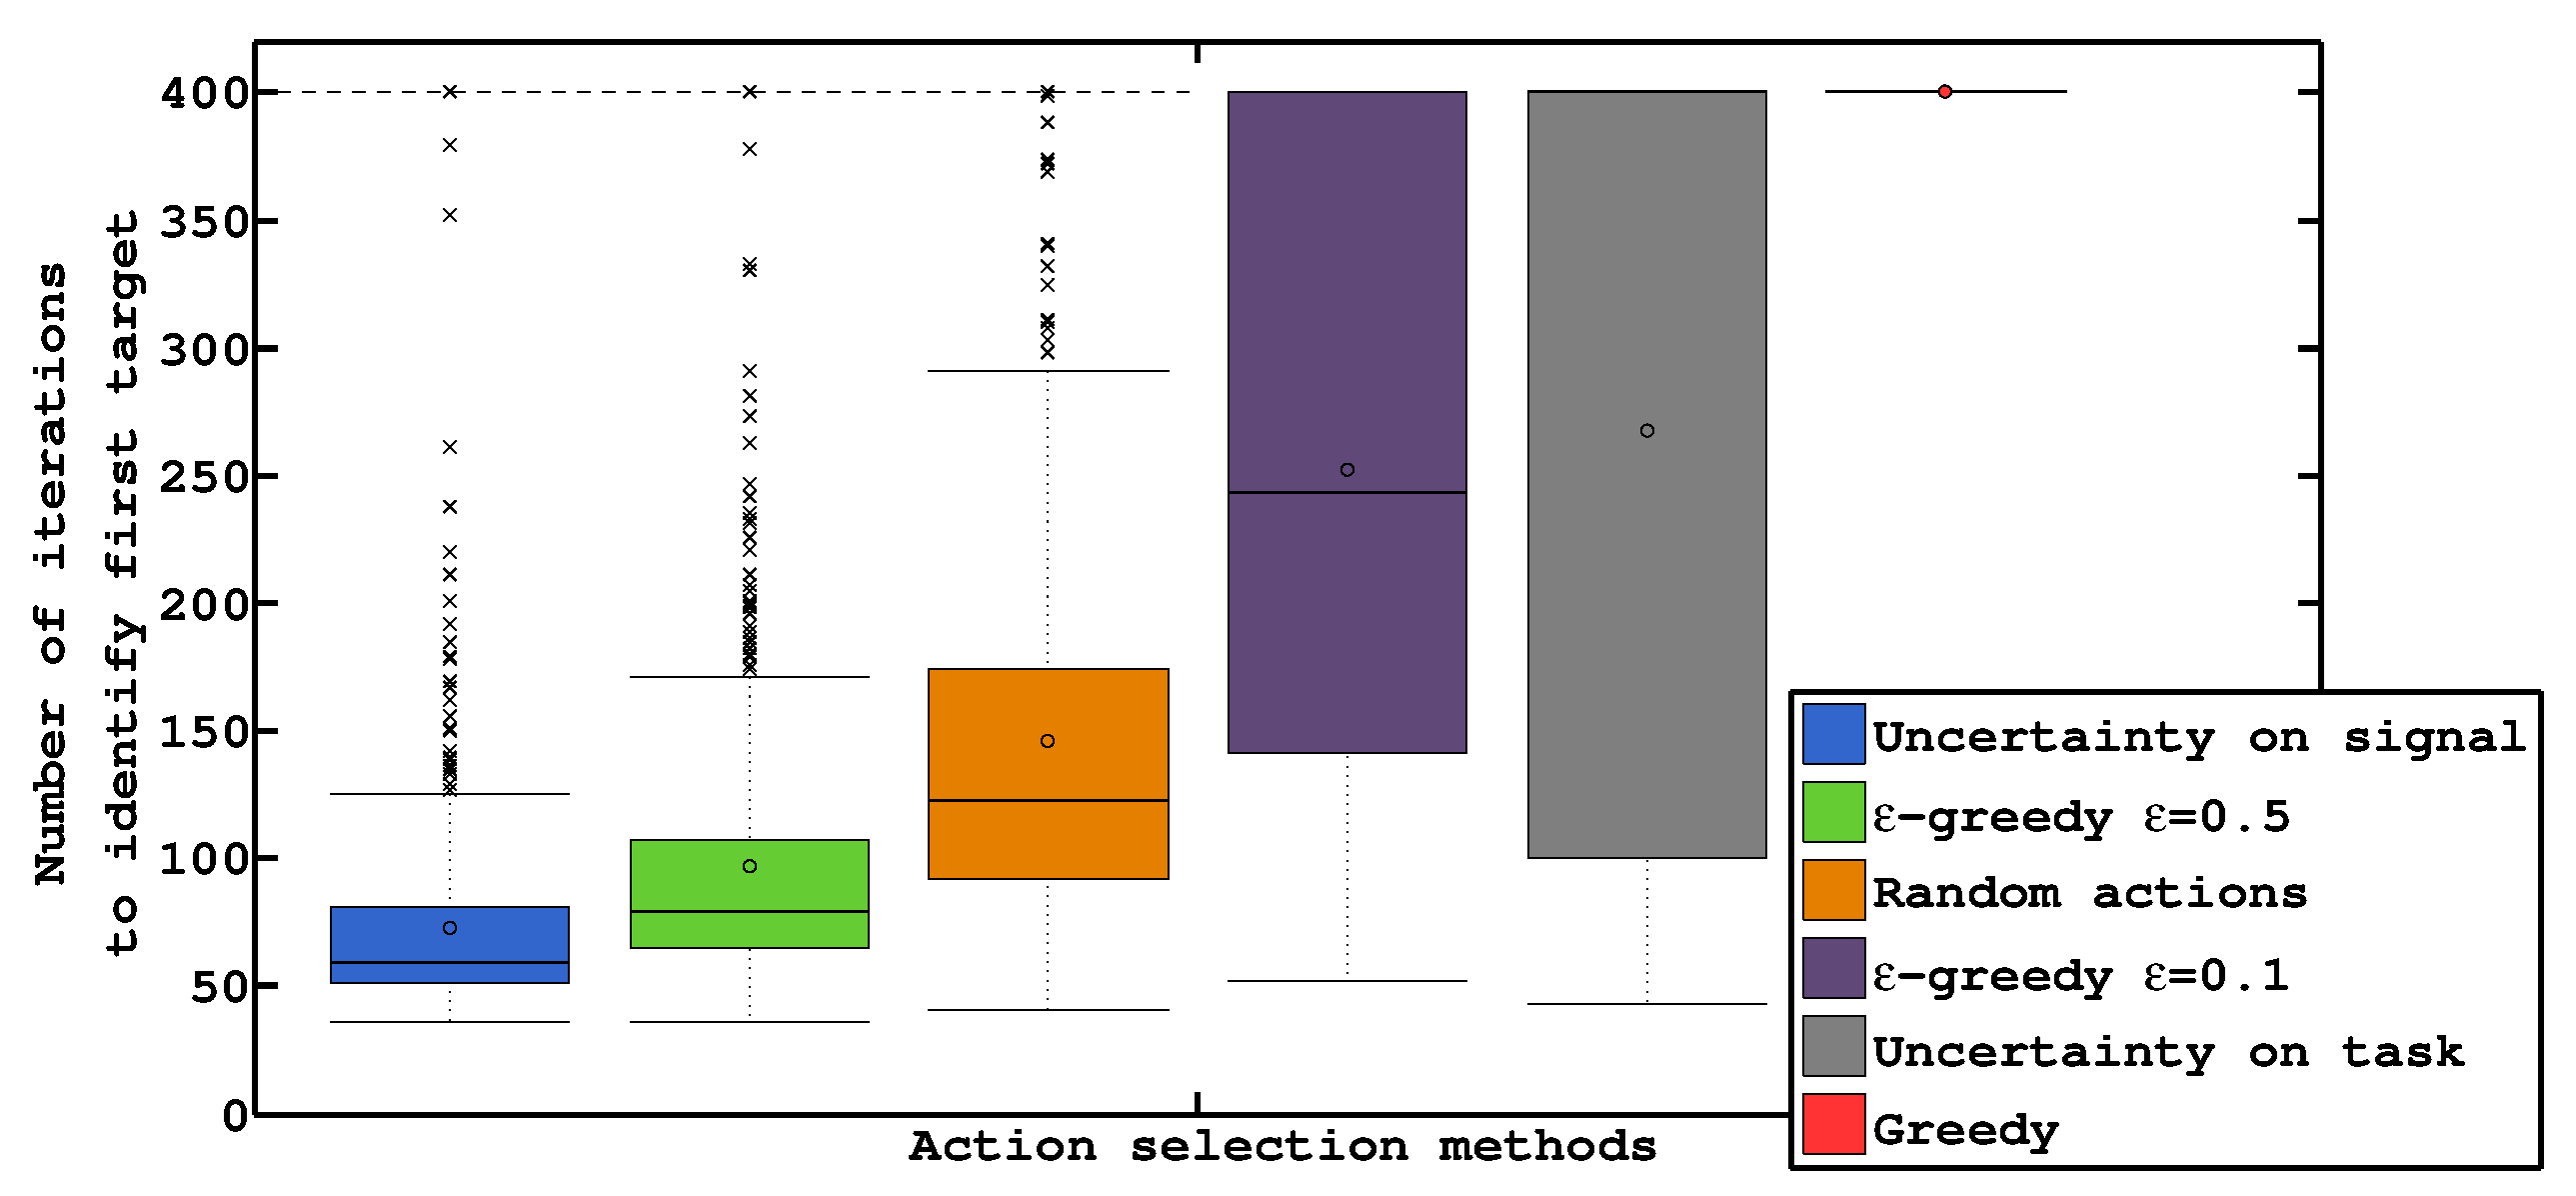
\includegraphics[width=\columnwidth]{\imgpath/plot_planning_first}
    \caption{Comparison of different exploration methods. Our proposed method, based on the uncertainty on the task and the signals interpretation, allows to lead the system to regions that improve disambiguation among hypotheses in a faster way. For the greedy method, all values were $400$ which indicates it never allowed to identify any task.}
    \label{fig:compplan}
\end{figure}

Figure~\ref{fig:compplan} shows the results averaged across subjects, runs and datasets. Values of $400$ means the confidence threshold was not reached after 400 iterations. Our proposed method, based on the uncertainty on the task and the signals interpretation, allows to lead the system to regions that improve disambiguation among hypotheses in a faster way. Trying to follow the most probable task does not allow the system to explore sufficiently (Greedy), and at least some random exploration is necessary to allow a correct identification of the task ($\varepsilon$-greedy). Assessing uncertainty only on the task performs poorly as it does not take into account the signal interpretation ambiguity inherent to our problem. The large variability in the results is mainly due to the large variations in classification accuracy across subjects and datasets. Given these results, the remainder of this section will only consider our proposed planning method.

\paragraph{Online re-estimation of classifier}
After identifying the first task, and following our approach, we continued running the system and measured how many tasks were identified after $400$ steps. The quality of our unsupervised method can be measured according to the percentage of labels correctly assigned (according to the ground truth label), see Figure~\ref{fig:percentageLabels}. In general, having dataset with classification accuracies higher than $75\%$ guaranteed that more than $90\%$ of the labels were correctly assigned. This result shows that our algorithm can also be used to collect training data for calibrating any other state-of-the-art error-related potentials classifier, but has the important advantage of controlling the device at the same time.

\begin{figure}[!ht]
    \centering
        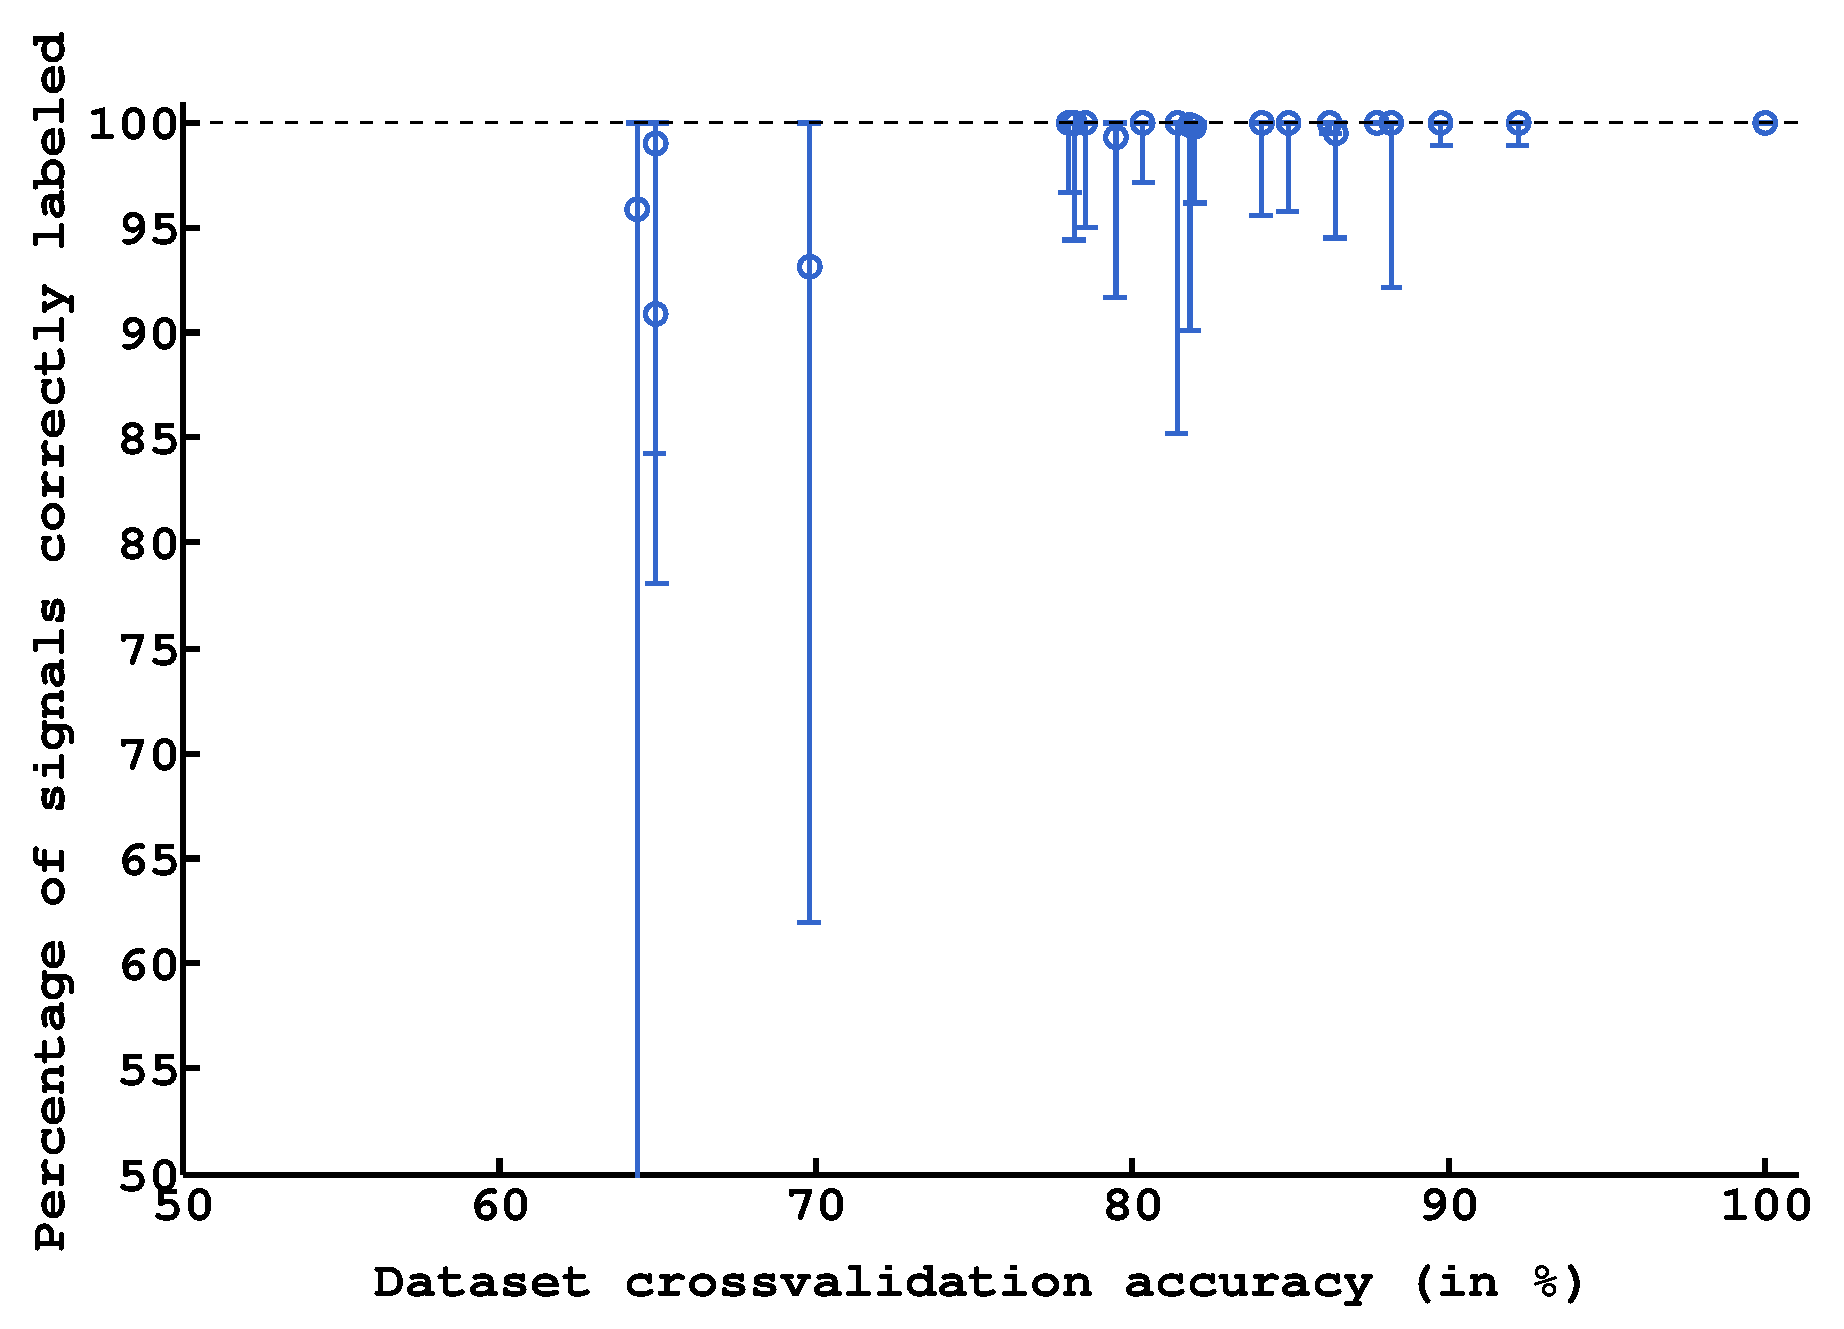
\includegraphics[width=\columnwidth]{\imgpath/plot_percent_label}
        \caption{Percentage of labels correctly assigned according to the ground truth label (the markers show the median values and the error bars the $2.5$th and $97.5$th percentiles). In general, having dataset with classification accuracies higher than $75\%$ guaranteed that more than $90\%$ of the labels were correctly assigned.}
        \label{fig:percentageLabels}
\end{figure}

Figure~\ref{fig:bhatta} demonstrates the advantage of switching to a Bayes filter method after identification of a first target instead of keeping the estimation given by the Bhattacharyya coefficient. On the one hand, Bhattacharyya coefficient works very well for small amounts of data because it directly compares model parameters. On the other hand, when there is sufficient data, training a classifier allows for a faster identification since the classifier makes a much harder decision when evaluating a new EEG signal.

\begin{figure}[!ht]
    \centering
        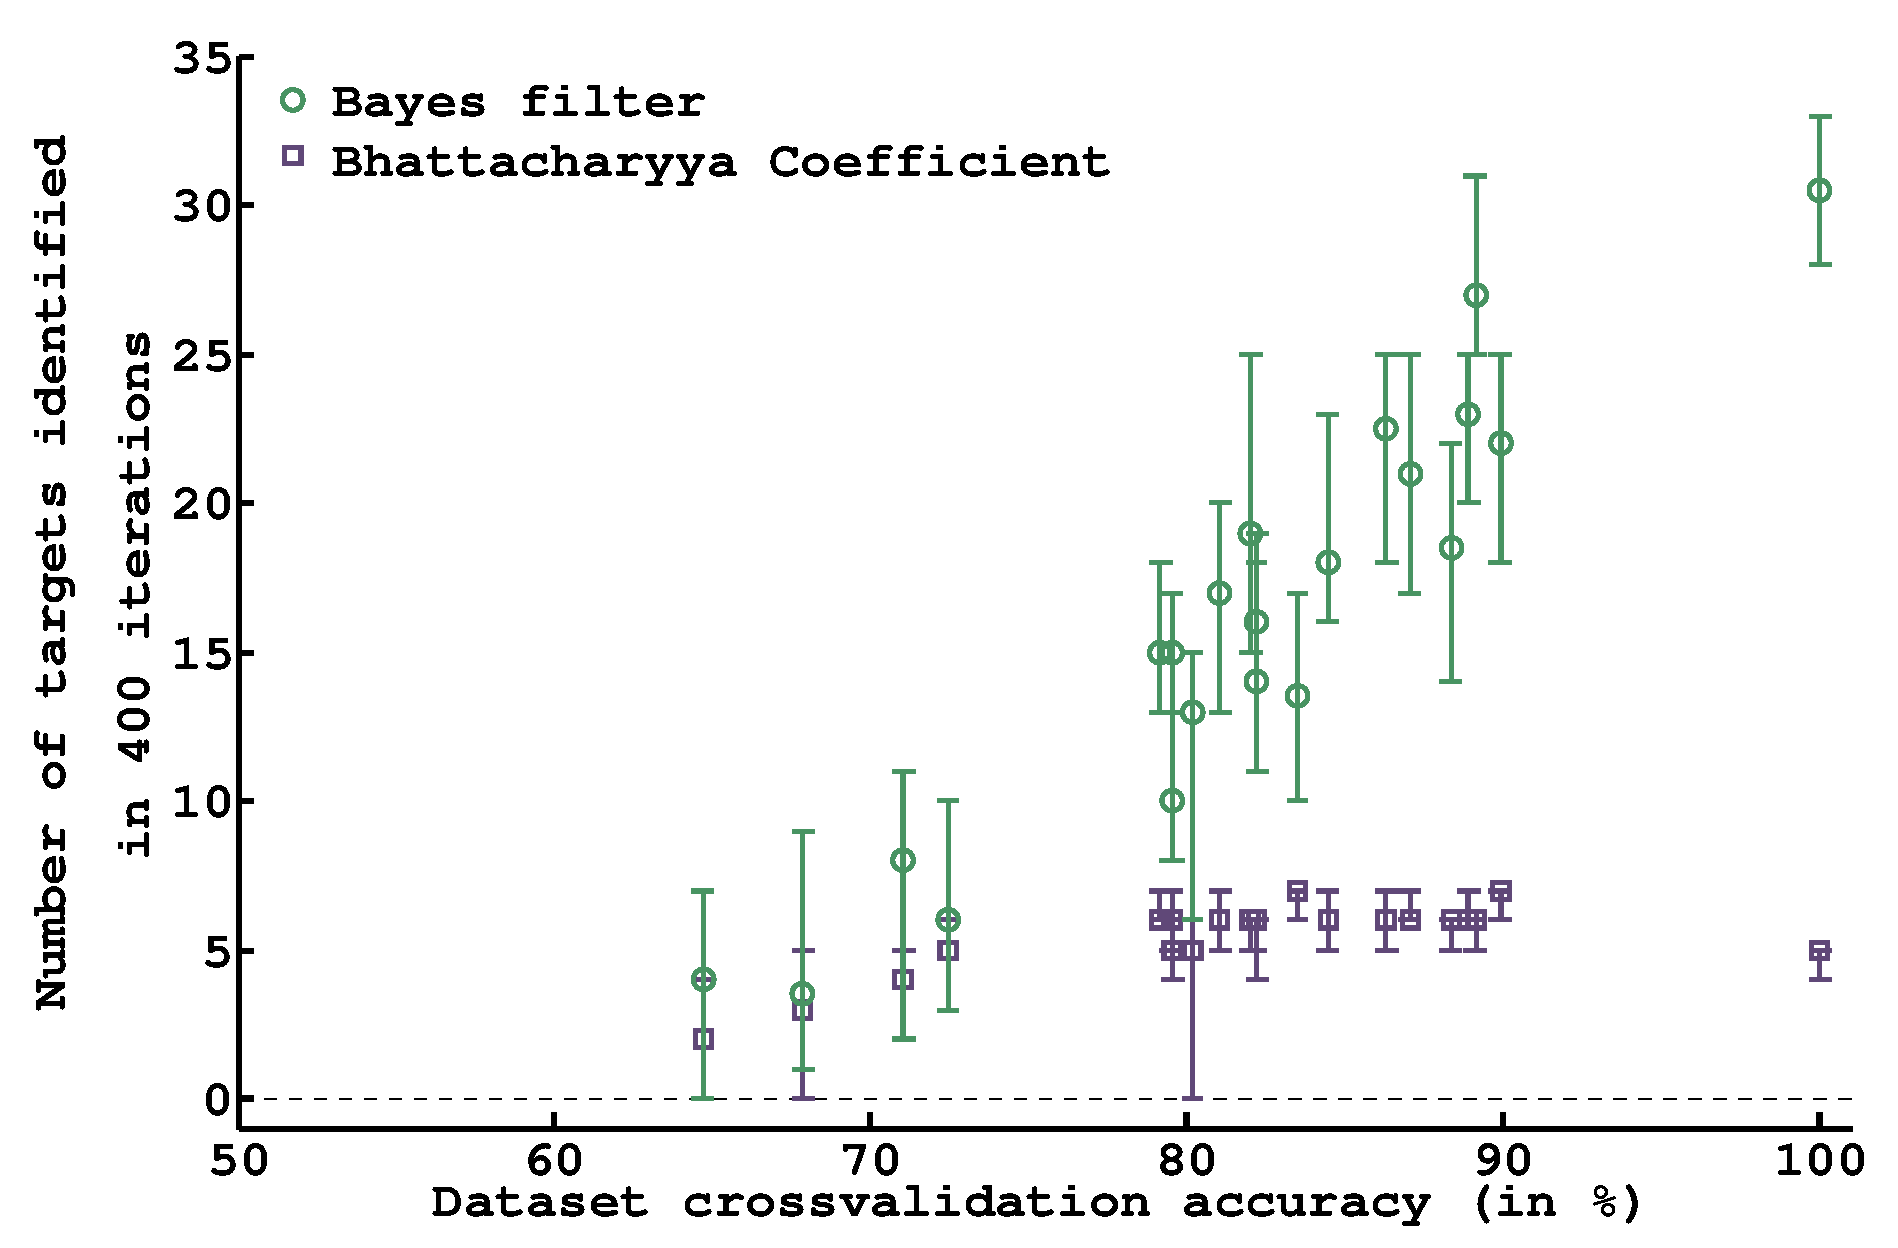
\includegraphics[width=\columnwidth]{\imgpath/plot_bhattha_vs_bayes}
        \caption{Number of targets correctly identified in $400$ iterations (the markers show the median values and the error bars the $2.5$th and $97.5$th percentiles). Comparison between switching to a Bayes filter method after identification of a first target instead of keeping the estimation given by the Bhattacharyya coefficient. The Bayes filter allows for a faster identification.}
        \label{fig:bhatta}
\end{figure} 

Figure~\ref{fig:avg_sum_400} shows the number of tasks correctly and incorrectly identified in $400$ iterations. For datasets of good qualities, we are able to identify more than $20$ tasks in $400$ iterations without the need for a calibration procedure (recap that previous works needed between 300 and 600 examples for the calibration phase \cite{chavarriaga2010learning,iturrate2010single}). The number of correctly identified tasks is strongly correlated to the quality of the dataset.

\begin{figure}[!ht]
    \centering
    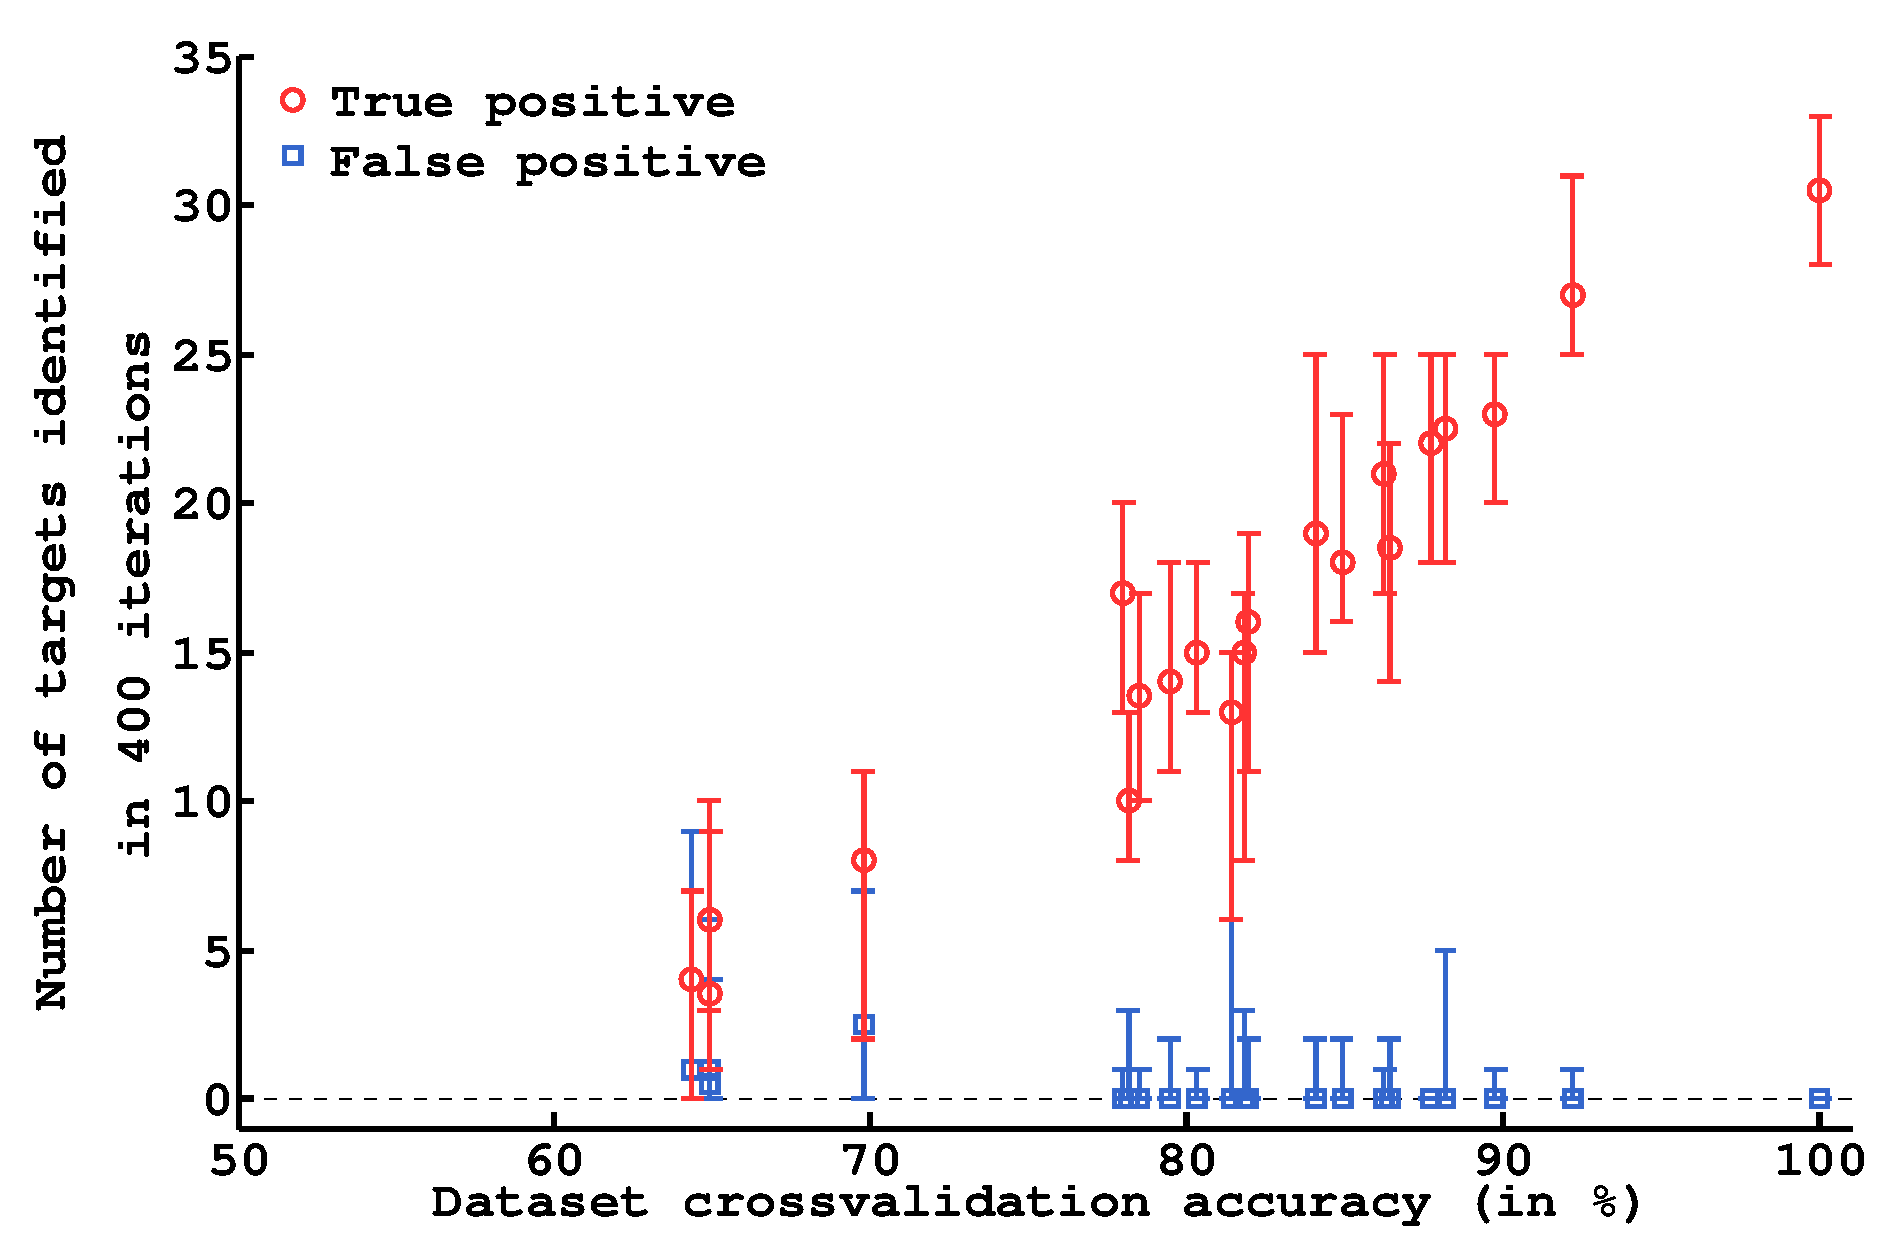
\includegraphics[width=\columnwidth]{\imgpath/plot_first400_reach} 
    \caption{Number of targets correctly and incorrectly identified in $400$ iterations (the markers show the median values and the error bars the $2.5$th and $97.5$th percentiles). For datasets of good qualities, we are able to identify more than $20$ tasks in $400$ iterations without the need for a calibration procedure.}
    \label{fig:avg_sum_400}
\end{figure} 

\paragraph{Robustness to Abrupt Changes in the Signals' Properties }
\label{CenterRobustnessToAbruptChangesInTheSignalsProperties}

We now want to determine whether the system is robust to changes in the signals' properties that occur when we change between different problem settings \cite{iturrate2013task}. We modeled this by changing from $Ti$ to $Tj$ ($i \neq j$) after $400$ steps, and then executing $400$ more steps from $Tj$. Both combinations ($T1$ to $T2$ and $T2$ to $T1$) were tested.

Figure~\ref{fig:stage2} shows the number of tasks identified depending on the classification accuracy on $Tj$ when training a classifier from dataset $Ti$. For abrupt changes which conserve a classification accuracy above $70\%$ on the new signals, our method, based on a limited size prior, is able to recover and solve more than $20$ tasks in $400$ iterations. For those cases where the accuracy change is too drastic, starting from scratch may be a better solution than relying on the adaptation properties of our algorithm.

\begin{figure}[!ht]
    \centering
    \includegraphics[width=\columnwidth]{\imgpath/plot_last400_reach}
    \caption{Number of targets correctly and incorrectly identified in $400$ iterations after an abrupt change in the signals properties (the markers show the median values and the error bars the $2.5$th and $97.5$th percentiles). For abrupt changes which conserve a classification accuracy above $70\%$ on the new signals, our method, based on a limited size prior, is able to recover and solve more than $20$ tasks in $400$ iterations.}
    \label{fig:stage2}
\end{figure}

\subsection{Online control}

This experiment evaluates if we can identify the task desired by the user even without an explicit calibration phase and without prior knowledge of the brain signals. The experiments were conducted with four subjects (aged between $25$ and $28$). Each subject was asked to mentally assess the agent's actions with respect to a given target. The system was not calibrated to decode the user EEG signals beforehand. Each subject performed $5$ runs, for each run a new target was randomly selected and provided to the user. There was an action every three seconds. Each run lasted $200$ actions, and the time between runs was around one minute.

The algorithm was able to identify the correct target for all runs of all the subjects, see Figure~\ref{fig:online_results}. There are strong variations among subjects but we note that our system identified each task in less iterations than a normal calibration phase requires (between 300 and 600 examples depending on the user performance \cite{chavarriaga2010learning,iturrate2010single}).

\begin{figure}[!htbp]
    \centering
    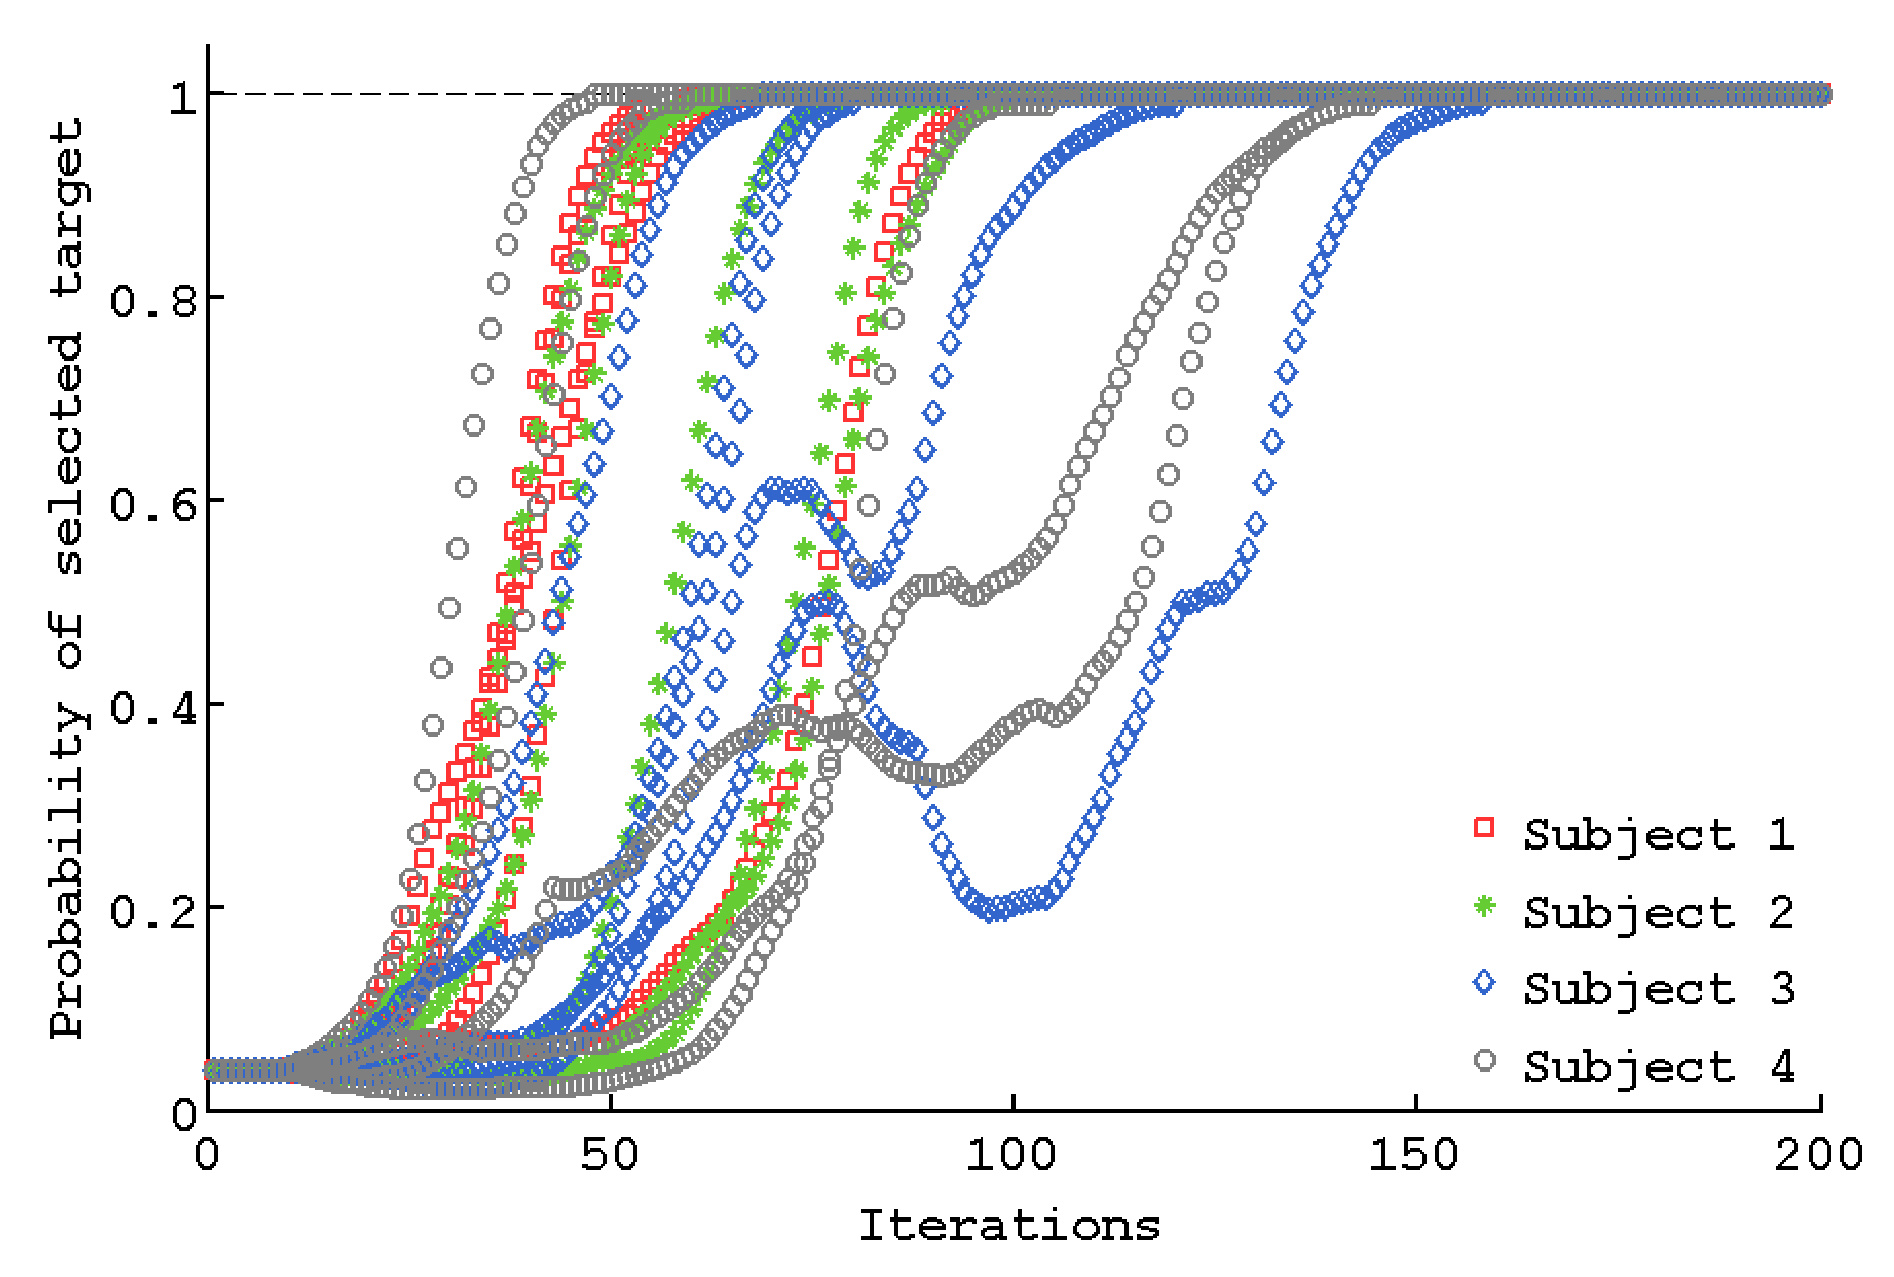
\includegraphics[width=\columnwidth]{\imgpath/plot_realevolution}    
    \caption{Results from the online experiment: Evolution of the probability of the correct task for each subject and run. The algorithm was able to identify the correct target for each subjects and runs in less than 200 iterations.}
    \label{fig:online_results} 
\end{figure}

Table~\ref{ch6tab:steps} shows for each subject and run the number of iterations needed to reach the confidence threshold for the subject selected target.

On average, the number of iterations needed to identify the target was of 85 $\pm$ 32.

\begin{table}[!ht]
\centering
\begin{footnotesize}
\begin{tabular}{r|rrrrr|r}
    %\toprule
    & \textbf{Run1} & \textbf{Run2} & \textbf{Run3} & \textbf{Run4} & \textbf{Run5} & \textbf{mean$\pm$std} \\\hline
    %\midrule
    \textbf{S1} & 95 & 62 & 56 & 60 & 64 & 67 $\pm$ 16 \\
    \textbf{S2} & 89 & 77 & 98 & 60 & 62  & 77 $\pm$ 17 \\
    \textbf{S3} & 68 & 80 & 118 & 76 & 157 & 100 $\pm$ 37 \\
    \textbf{S4} & 98 & 142 & 57 & 142 & 47 & 97 $\pm$ 45 \\
    %\bottomrule
\end{tabular}
\end{footnotesize}
  \caption{Results from the online experiment: Number of iterations needed to identify the correct target for each subject and run. On average, the number of iterations needed to identify the target was of 85 $\pm$ 32.}
  \label{ch6tab:steps}
\end{table}

%%%%%%%%%%%%%%%%%%%%%%%%%%%%%%%%%%%%%%%%%%%%%%
%%%%%%%%%%%%%%%%%%%%%%%%%%%%%%%%%%%%%%%%%%%%%%
%%%%%%%%%%%%%%%%%%%%%%%%%%%%%%%%%%%%%%%%%%%%%%
%%%%%%%%%%%%%%%%%%%%%%%%%%%%%%%%%%%%%%%%%%%%%%
%%%%%%%%%%%%%%%%%%%%%%%%%%%%%%%%%%%%%%%%%%%%%%
\section{Discussion}

We introduced a novel method for calibration-free BCI based control of sequential tasks with feedback signals. The method provides an unsupervised way to train a decoder with almost the same performance as state-of-the-art supervised classifiers, while keeping the system operational and solving the task requested by the user since the beginning. 
%
The intuition for our method is that the classification of the brain signals is easier when they are interpreted according to the task desired by the user. The method assumes a distribution of possible tasks and relies on finding which pair of decoder-task has the highest expected classification rate on the brain signals. 


The algorithm was tested with real online experiments, showing that the users were able to guide an agent to a desired position by mentally assessing the agent's actions and without any explicit calibration phase. Offline experiments show that we can identify an average of 20 tasks in 400 iterations without any calibration, while in previous works the calibration phase used between 300 and 600 examples. To improve the efficiency of the algorithm, we introduced a new planning method that uses the uncertainty in the decoder-task estimation. Finally, we analyzed the performance of the system in the presence of abrupt changes in the EEG signals. Our proposed method was able to adapt and reuse its learned models to the new signals. Furthermore, in those cases when the transfer is not possible, our method can still be used to recalibrate the system from scratch while solving the task.

A current limitation of the work is the need for a finite set of task hypotheses. This limitation could be solved by the use of a combination of particle filter and regularization on the task space. Additionally, our method can not dissociate fully symmetric hypotheses, e.g.\ right and left most state of our 1D grid world (Fig. \ref{fig:GM}), as the interpretation of feedback signals will also be symmetric and therefore as likely. This latter problem can be solved by redefining the set of hypotheses or the action set, for instance by adding a ``stop'' action valid only at the target state.

This work opens a new perspective regarding the global challenge of interacting with machines. It has application to many interaction problems which requires a machine to learn how to interpret unknown communicative signals. A promising avenue, outside the BCI field, lies in human robot interaction scenarios where robots must learn from, and interact with, many different users who have their own limitations and preferences.




%%%%%%%%%%%%%%%%%%%%%%%%%%%%%%%%%%%%%%%%%%%%%%
%%%%%%%%%%%%%%%%%%%%%%%%%%%%%%%%%%%%%%%%%%%%%%
%%%%%%%%%%%%%%%%%%%%%%%%%%%%%%%%%%%%%%%%%%%%%%
%%%%%%%%%%%%%%%%%%%%%%%%%%%%%%%%%%%%%%%%%%%%%%
%%%%%%%%%%%%%%%%%%%%%%%%%%%%%%%%%%%%%%%%%%%%%%
\section{Continuous state space}


In this section we extend our algorithm to a more complex scenario by considering a continuous world, more complex reward functions and the use of both feedback and guidance instructions. We investigate how our algorithm scales to such problem and how different exploration strategies perform.

\subsection{Experimental System}

We now illustrate the application of our algorithm in a more complex problem. This problem is known in the reinforcement learning literature as the \emph{puddle world}. The puddle world consist in a continuous-state MDP in which an agent must reach a goal region while avoiding a penalty region.
% 
In this work we consider a 2 dimensional puddle world with each dimension ranging between 0 and 1. Agent actions are discrete and represent steps in either North, South, East, West direction. One step length is sampled from a normal distribution of mean 0.1 and standard deviation 0.01.

As in the previous experiment, we consider speech as the modality for interacting with the robot and we reuse the dataset used in section~\ref{sec:First}. The interaction scheme is turn taking, where the agent is performing an action and wait for a feedback or guidance signal to continue (see section \ref{sec:mixing}). We only consider a Gaussian classifier.

\subsubsection{Task Representation}
To define the set of possible tasks we project a 5x5 regular grid on top of the continuous world. One task is represented by a +1 reward in one of the 25 projected squares and a -100 reward in three consecutive (vertically or horizontally) squares. +1 and -100 area can not overlap (see figure~\ref{UncertaintyMap}(E) for an example). The set of possible task is defined as all possible combination of such reward function, for a total of 660 hypothesis. 

We use the MDP framework to compute the corresponding policies. The world being continuous we use the tile coding function approximation \cite{sutton1998reinforcement}, with 10 overlapping 50x50 regular grids. %tillins. 
A Q-Learning algorithm \cite{watkins1992q} is used to compute the Q-Values, with a discount rate of 0.99 and a learning rate of 0.01. The hypothesis policies are then defined as greedy according to the Q-Values.

\subsubsection{Exploration strategies}

We will investigate four different agent behaviors. 1) random, 2) $\epsilon$-greedy, 3) myopic uncertainty based exploration, which aim at selecting the action that is the most uncertain in the current state, and 4) full uncertainty based exploration which requires an uncertainty map to decide what to explore next, as presented in Section~\ref{sec:Planning}. 

As we are in a continuous domain we can not compute the full uncertainty for each state as presented in Section \ref{sec:ExplorationMethod}, we therefore approximate this process. Extensions already exist for the continuous state problem \cite{nouri2010dimension,Hester13aamas} and we will rely on a sampling based method. One hundred random states are generated and evaluated in terms of task and instruction uncertainty as described in Algorithm~\ref{alg:u}. Each sampled state is associated to a reward value proportional to its uncertainty which is propagated to neighborhood states by using a fixed Gaussian kernel. We use as amplitude the uncertainty value and a diagonal covariance matrix of value 0.01. The resulting approximated uncertainty map is then used as a reward function in a new MDP problem. By solving this problem, using for instance Q-Learning, the agent plans actions to visit the most uncertain regions. The system can then run an $\epsilon$-greedy policy on this solution. In the following experiment, the agent will use an exploration ratio $\epsilon$ equal to $0.1$.

\subsubsection{Feedback and Guidance Model}
\label{sec:advancedModel}


\subsection{Mixing feedback and guidance}
\label{sec:mixing}

The previously defined teaching signal model limits the use of only feedback or only guidance instruction. Such limitation can be restrictive for the user, we will now consider the case where teachers can use both, i.e. $z \in \{F \cup G\}$. Extending our algorithm to cases where possible meanings include both feedback and guidance requires a probabilistic model of how the teacher distribute feedback and guidance signals. This model must hold the following property $\sum_{i \in \{F \cup G\}} p(z = i|s,a,\hat{\xi})~=~1$. We define a variable $\beta$ that represents the probability of the user providing a feedback signal at each step, i.e. $p(z \in F) = \beta$, which implies $p(z \in G) = 1 - \beta$. 

In \cite{macl11simul} the agent was estimating such protocol parameters from the interaction. In this work we will assume such parameter is known in advance (see Section~\ref{sec:advancedModel}) and further assume it does not depend on the task or on the state of the robot. 
%
Under this new definition we can change the likelihood function to:
%
\begin{eqnarray}
\L_i &=&  p(n_i|s_i,a_i,\hat{\xi},\theta)\nonumber\\
%               &=& \sum_{j} p(n_i|z = j,s_i,a_i,\hat{\xi},\theta)~p(z = j|s_i,a_i,\hat{\xi},\theta)    \nonumber\\
                &=& \sum_{j} p(n_i|z = j,\theta)~p(z = j|s_i,a_i,\hat{\xi}) \nonumber\\
                &=& \sum_{j} p(n_i|z = j,\theta)~w_{ij}^{\hat{\xi}}
                \label{eq:likmix}
\end{eqnarray}
%
with :
%
\begin{eqnarray}
    w_{ij}^{\hat{\xi}} = 
        \begin{cases} 
            \beta~p(z|s_i,a_i,\hat{\xi}) &\mbox{for } z \in F \\
            (1- \beta)~p(z|s_i,\hat{\xi}) & \mbox{for } z \in G
        \end{cases} 
\end{eqnarray}

We consider both feedback and guidance instruction simultaneously. Extending our algorithm to cases where possible meanings include both feedback and guidance requires a probabilistic model of how the teacher distribute feedback and guidance signals. We will use the mixing model described in Section~\ref{sec:mixing} with the individual feedback and guidance model as describe in Section~\ref{sec:fisrtFrame} and a mixing ratio $\beta$ of 0.5. It means that the user is expected to deliver feedback and guidance signals at a similar rate.


\subsection{Results}

We present results from 75 runs of our experiment, where for each run we randomly choose a task to teach from the set of hypothesis as well as the initial state of the agent. For each experiment, we compute the likelihoods every 15 steps and performs a total of 35 updates, for a total of 525 iterations. Figure~\ref{Rmax} shows the average evolution of the taught task hypothesis likelihood.

\begin{figure}[!htbp]
  \centering
  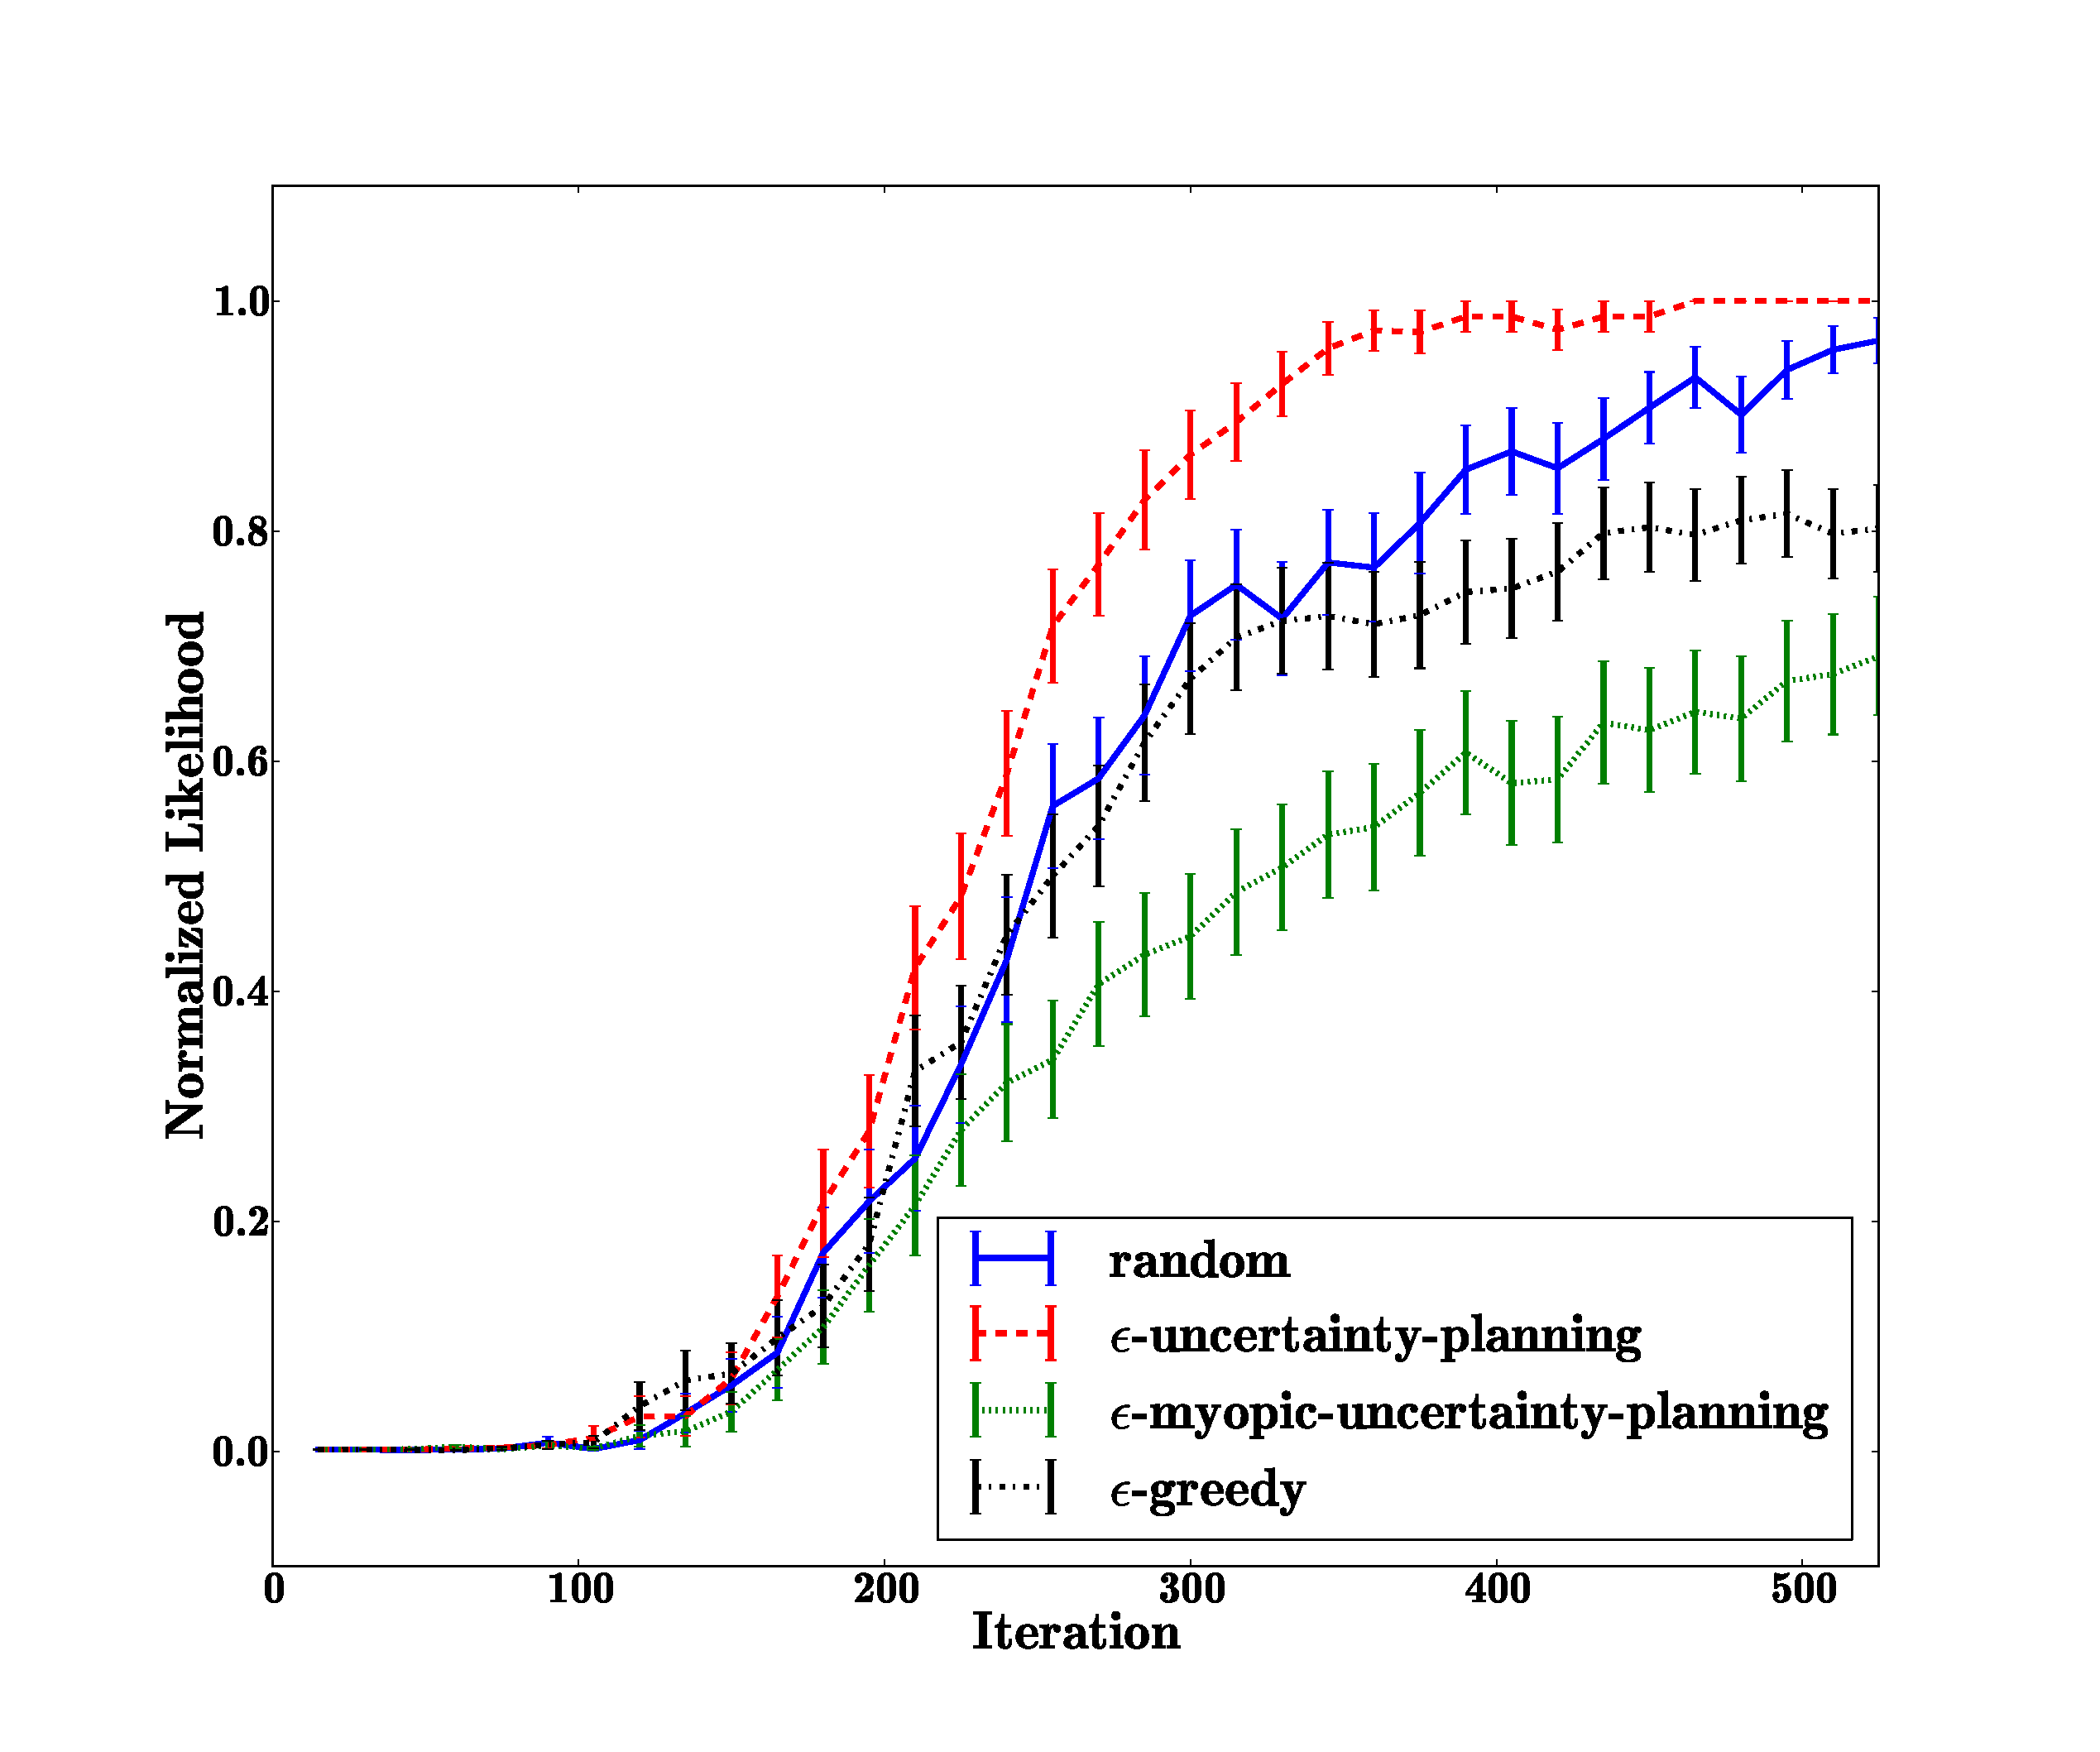
\includegraphics[width=\columnwidth]{\imgpath/continuous}
  \caption{Taught hypothesis normalized likelihood evolution (mean + standard error) thought iteration using Gaussian classifer. Comparaison of different exploration strategies. Uncertainty based exploration method, which plan on the long term, performs significantly better.}
  \label{Rmax}
\end{figure}

Results from figure~\ref{Rmax} show that our algorithm can learn a task in a continuous world from unknown and noisy instructions whose possible meanings are both feedback and guidance and 10\% of the instructions were teaching mistakes. The uncertainty based planning strategy outperforms random action selection. Interestingly, myopic uncertainty based strategy, which is also based on both task and signal uncertainty, is not efficient. This result illustrates some of the issues discussed in section~\ref{sec:Planning}, when considering the agent as not being able to teleport, long term planning is more suited to explore efficiently the state space. 

As expected $\epsilon$-greedy performs less efficiently than in the first setup. This is due to the properties of our new set of hypothesis where many hypothesis shared an identical positive reward area but have different puddle zone.

Figure~\ref{UncertaintyMap} shows the evolution of the estimated uncertainty map for one run of the experiment. For each uncertainty map, the agent plans its actions to reach a maximal uncertainty region. The maximum uncertainty value decreases as the agent is correctly estimating the task.

\begin{figure}[!htbp]
  \centering
      \begin{subfigure}[b]{0.35\columnwidth}
          \centering
          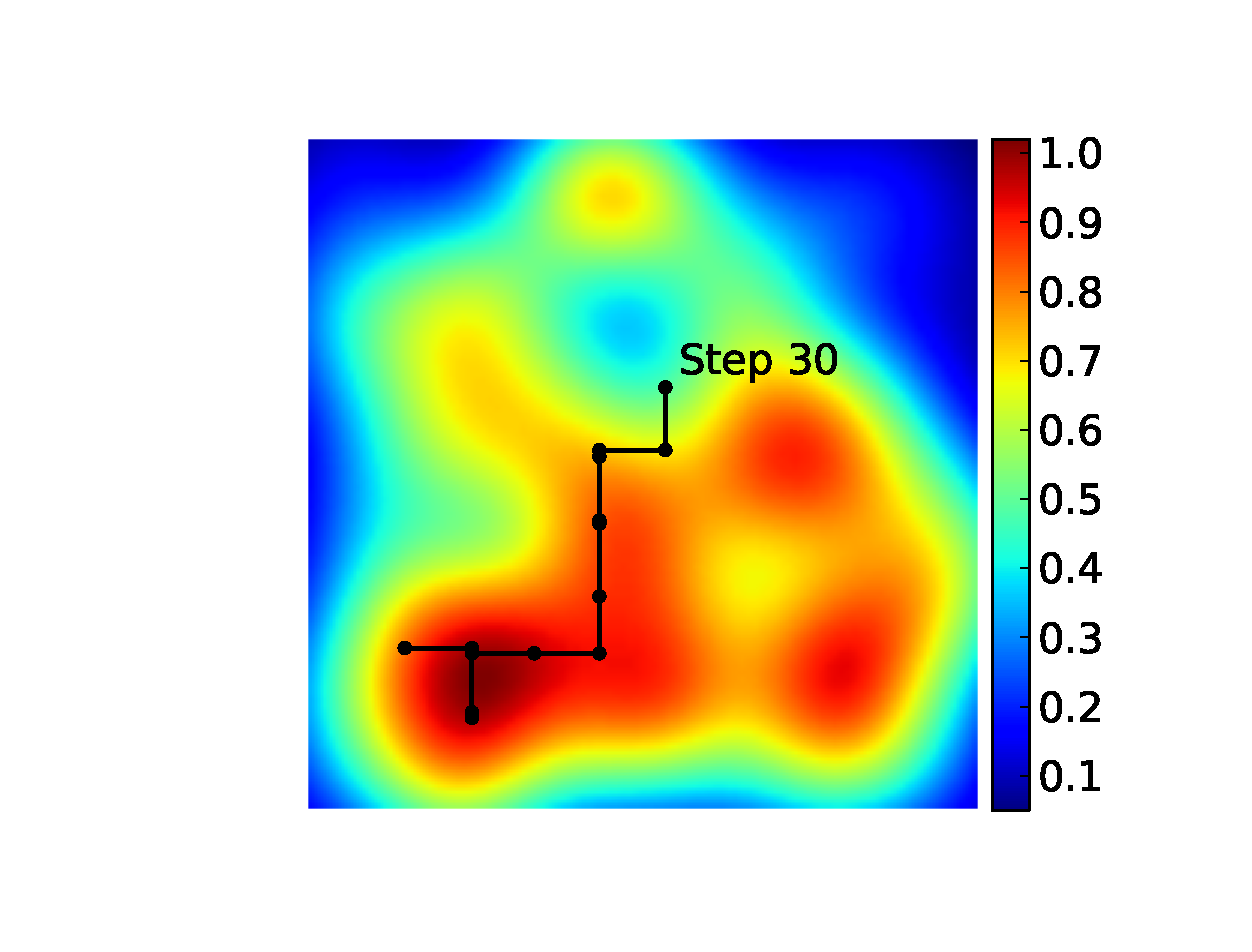
\includegraphics[trim=5cm 1.5cm 1.5cm 1.5cm, clip=true, width=\columnwidth]{\imgpath/30}
          \caption{After 30 iterations.}
          \label{fig:30}
      \end{subfigure}
      \begin{subfigure}[b]{0.35\columnwidth}
          \centering
          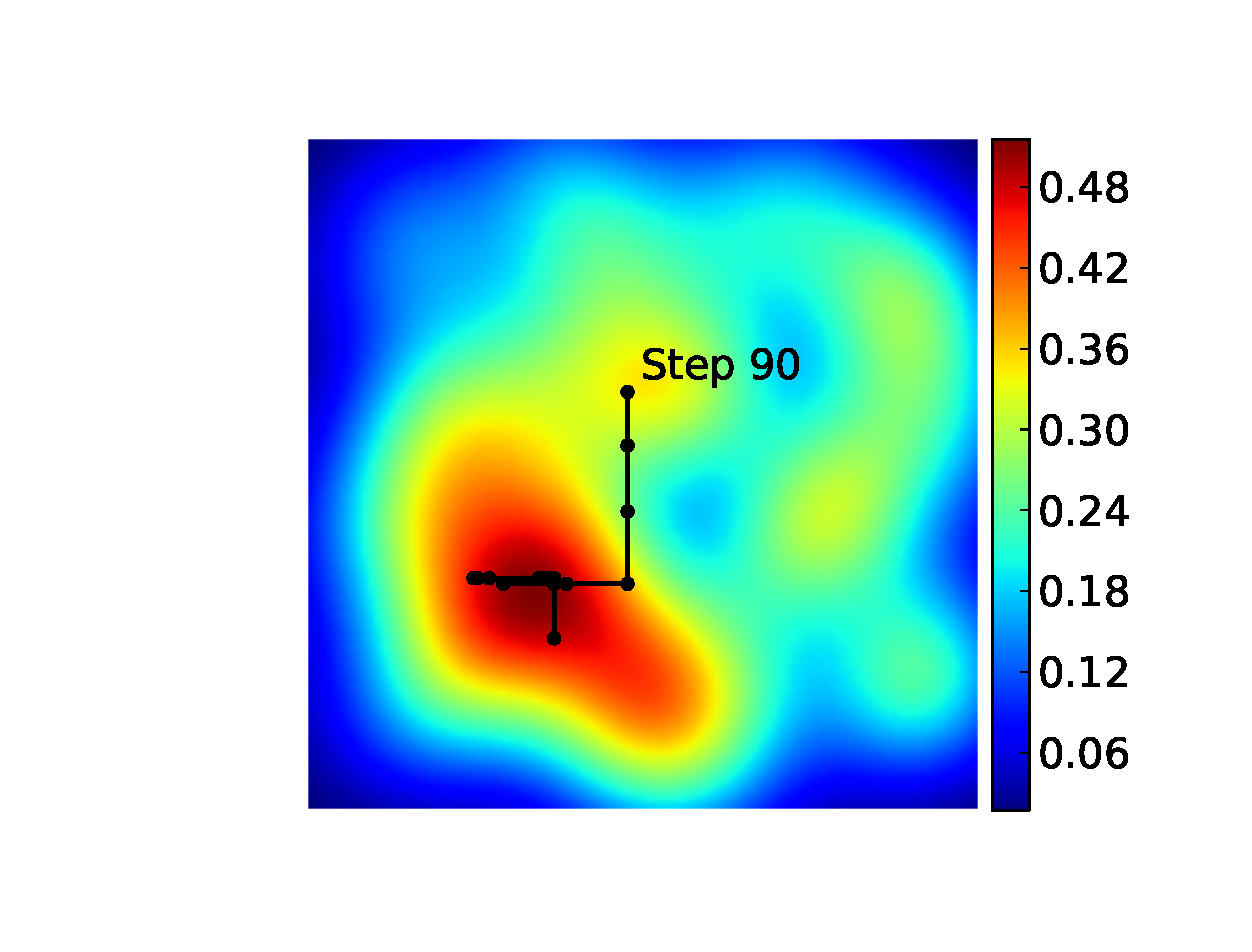
\includegraphics[trim=5cm 1.5cm 1.5cm 1.5cm, clip=true, width=\columnwidth]{\imgpath/90}
          \caption{After 90 iterations.}
          \label{fig:90}
      \end{subfigure}\\
      \begin{subfigure}[b]{0.35\columnwidth}
          \centering
          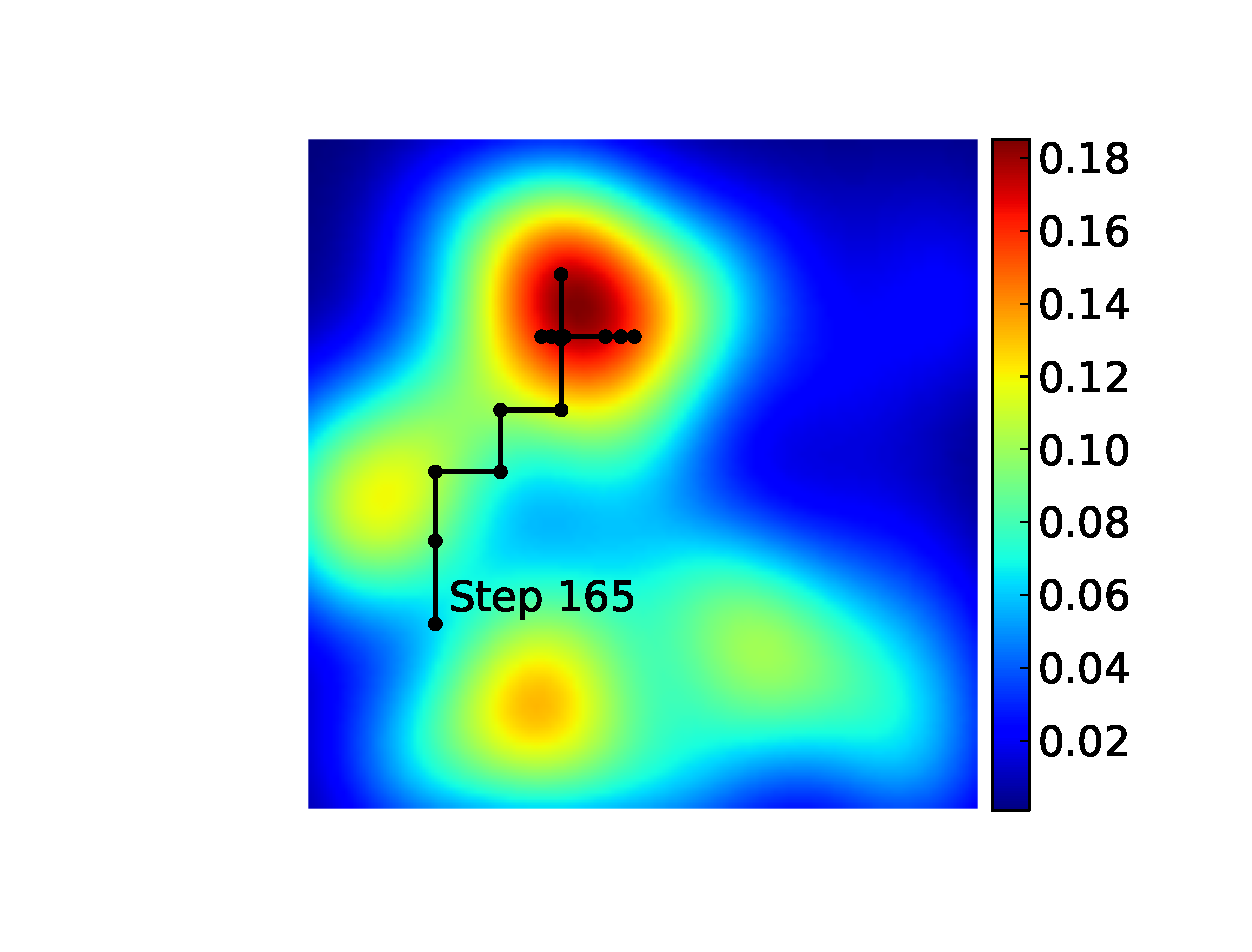
\includegraphics[trim=5cm 1.5cm 1.5cm 1.5cm, clip=true, width=\columnwidth]{\imgpath/160}
          \caption{After 165 iterations.}
          \label{fig:165}
      \end{subfigure}
      \begin{subfigure}[b]{0.35\columnwidth}
          \centering
          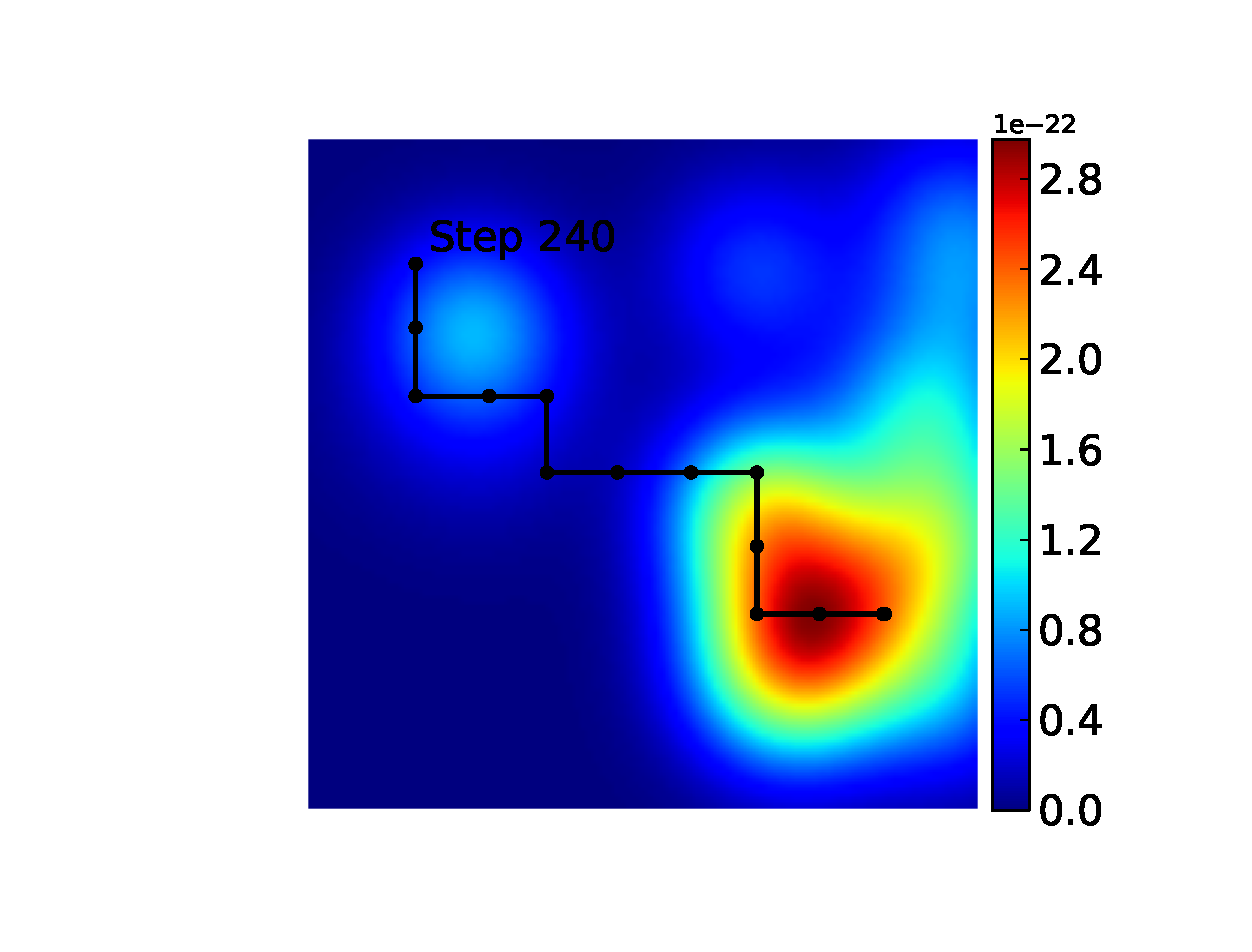
\includegraphics[trim=5cm 1.5cm 1.5cm 1.5cm, clip=true, width=\columnwidth]{\imgpath/240}
          \caption{After 240 iterations.}
          \label{fig:240}
      \end{subfigure}\\
      \begin{subfigure}[b]{0.25\columnwidth}
          \centering
          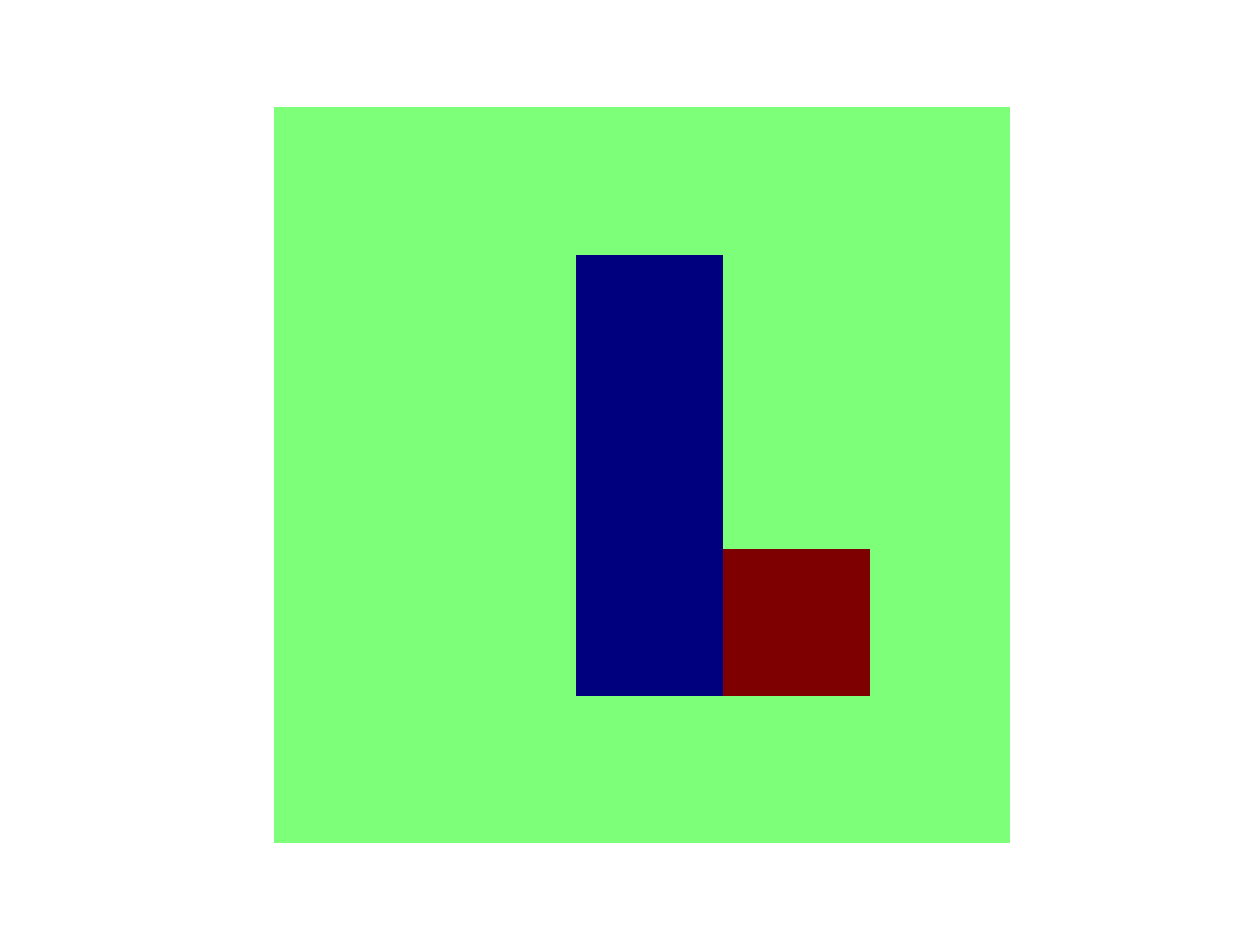
\includegraphics[trim=4cm 1cm 3.5cm 1cm, clip=true, width=\columnwidth]{\imgpath/puddle}     
          \caption{Puddle world used by the teacher.}
          \label{fig:puddle}
      \end{subfigure}
      \begin{subfigure}[t]{0.45\columnwidth}
          \centering
          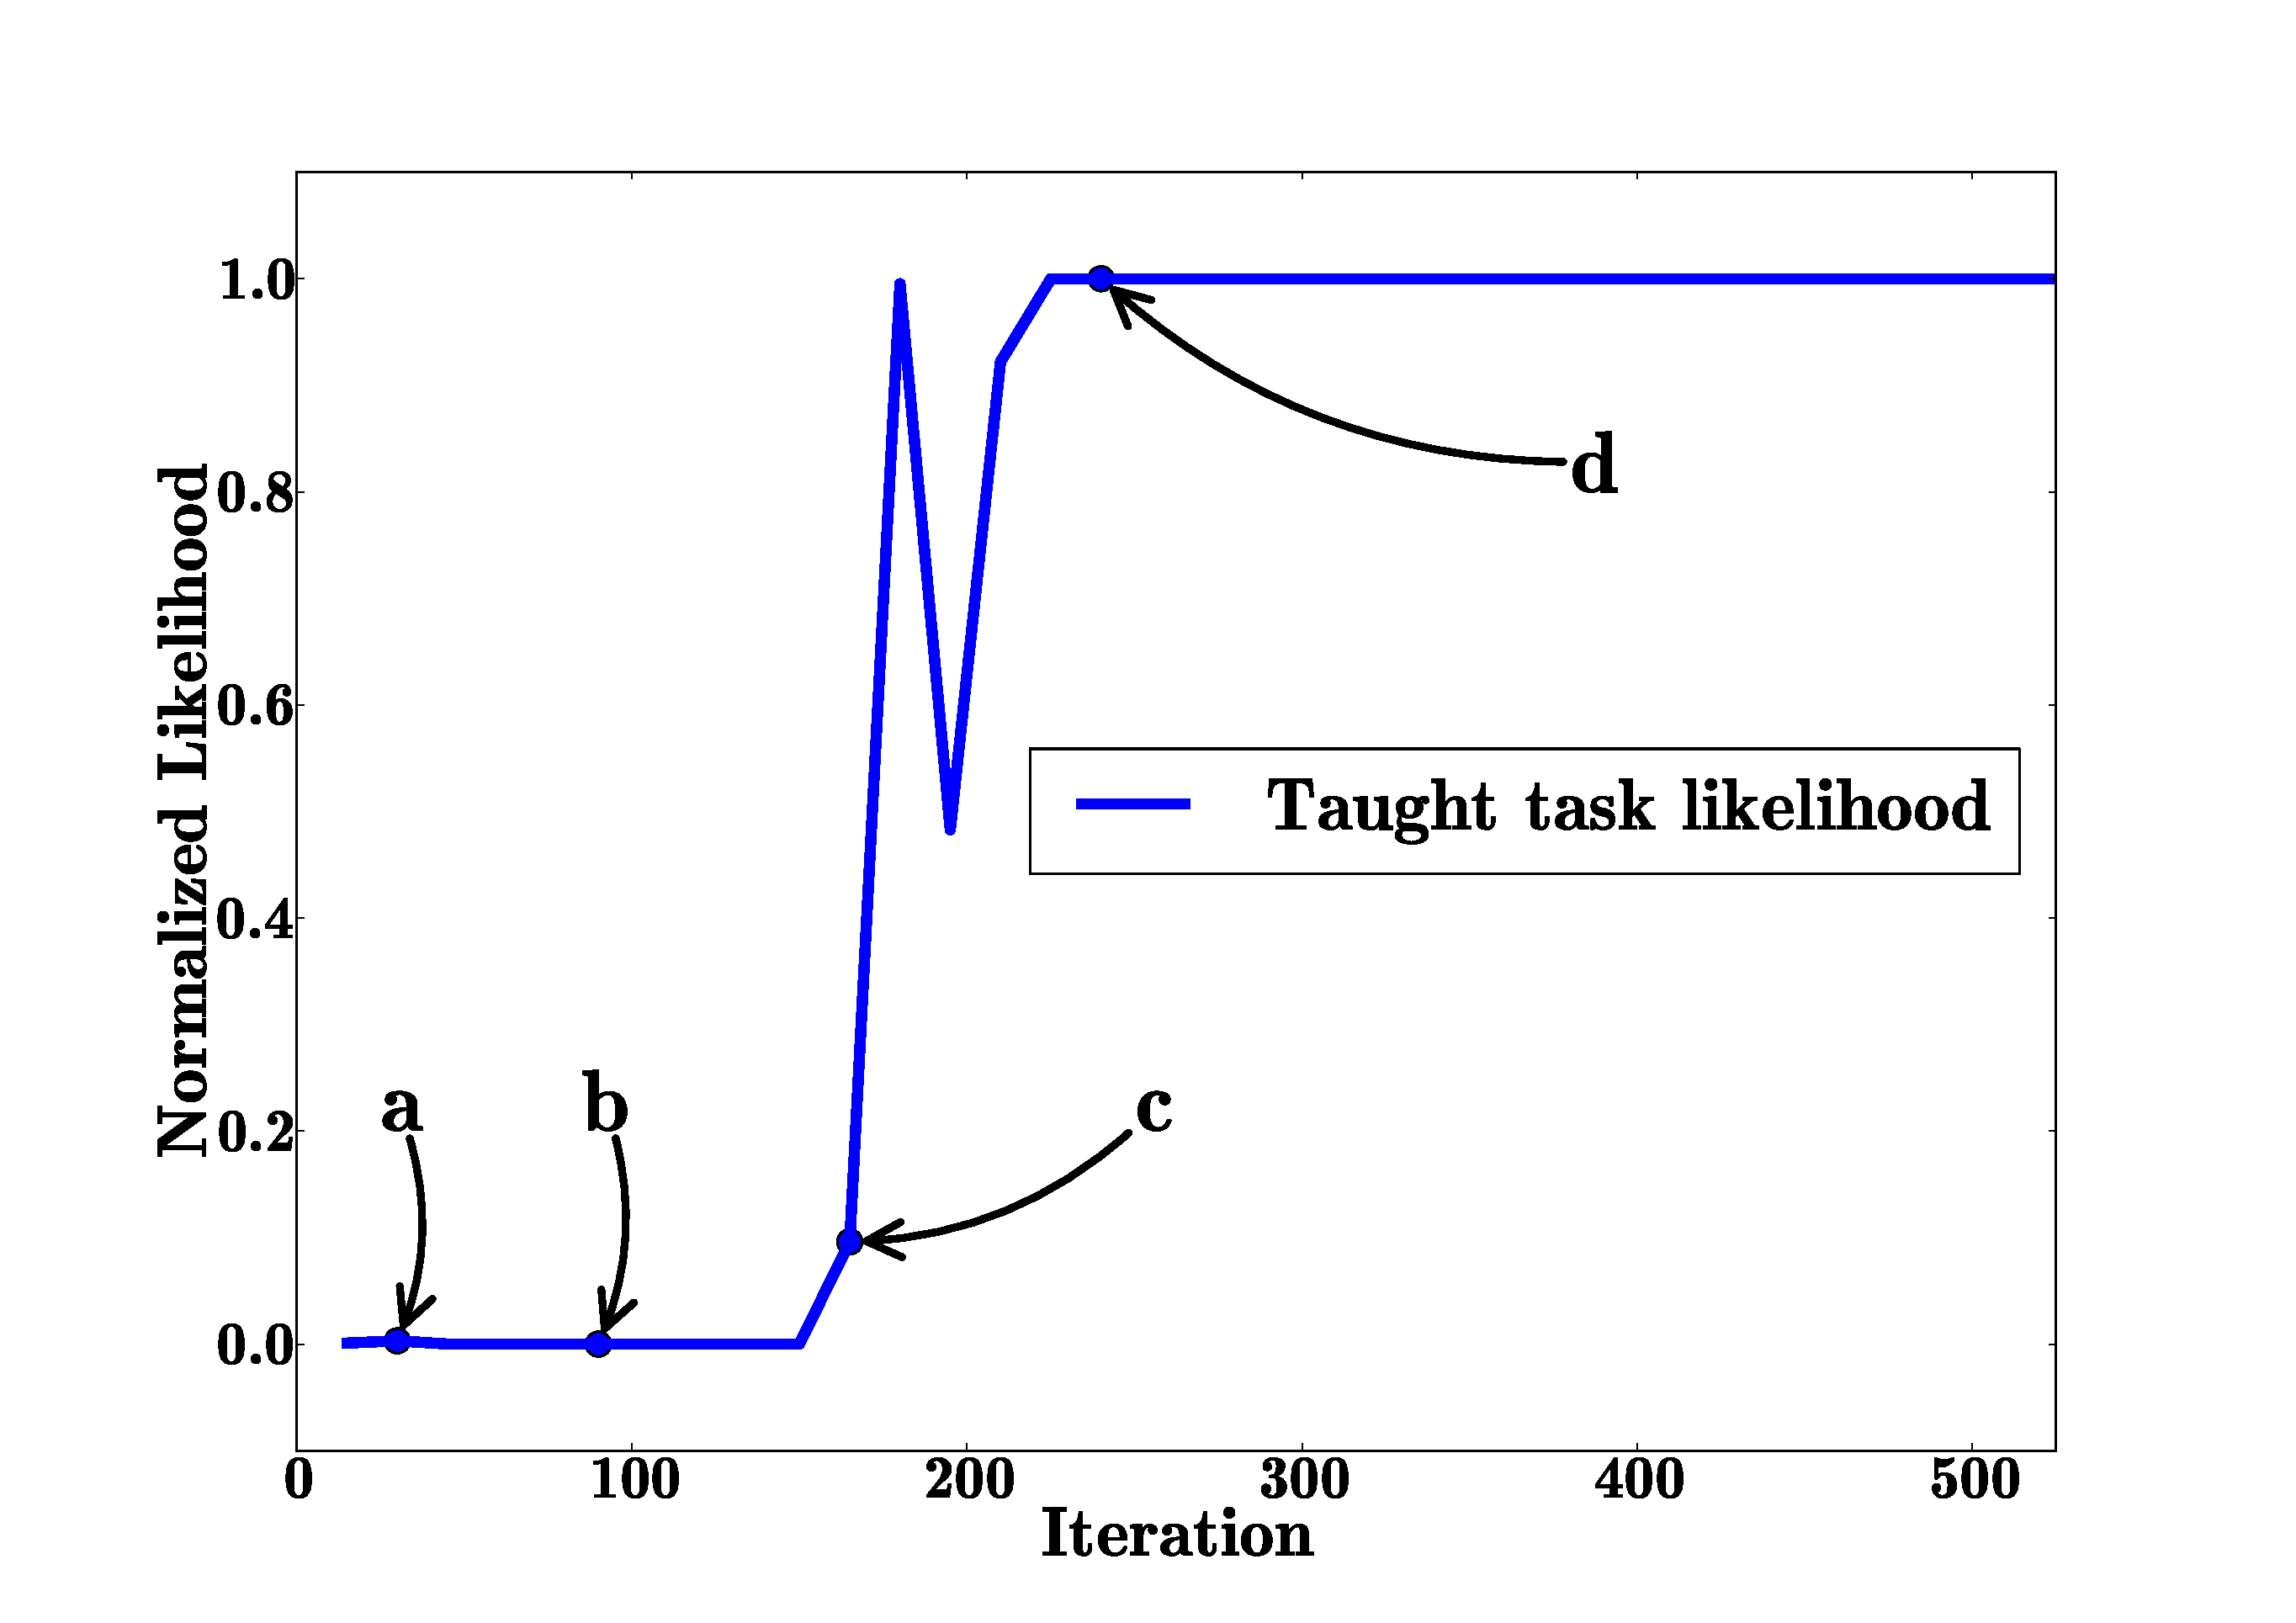
\includegraphics[trim=2cm 1cm 3cm 2cm, clip=true, width=\columnwidth]{\imgpath/evo}
          \caption{Taught hypothesis normalized likelihood evolution.}
          \label{fig:evo}
      \end{subfigure}
        
  \caption{Log Uncertainty maps after a) 30, b) 90, c) 165 and d) 240 iterations. e) shows the puddle world choosen by the teacher and f) shows the learning progress and the frame associated to each of the uncertainty map. In order to display the differences between log values, we bounded the colormap between -5 and 0, which correspond to uncertainty values between 0.0067 and 1. Some log values, especially for d), are lower than -5 and are displayed in the same color as -5. Best shown in color.}
  \label{UncertaintyMap}
\end{figure}

%%%%%%%%%%%%%%%%%%%%%%%%%%%%%%%%%%%%%%%%%%%%%%
%%%%%%%%%%%%%%%%%%%%%%%%%%%%%%%%%%%%%%%%%%%%%%
%%%%%%%%%%%%%%%%%%%%%%%%%%%%%%%%%%%%%%%%%%%%%%
%%%%%%%%%%%%%%%%%%%%%%%%%%%%%%%%%%%%%%%%%%%%%%
%%%%%%%%%%%%%%%%%%%%%%%%%%%%%%%%%%%%%%%%%%%%%%
\section{Continous set of hypothesis}
\label{chapter:limitations:continoushypothesis}

a simple particle filter

How to leverage from the finite set of hypothesis constraint? A potential avenue is to use a combination of particle filter and regularization on the task space.

\paragraph{Pre-defined finite set of tasks and instruction meanings} In order to make the learning problem tractable, it was assumed in this article that the robot learner knows that the task to be learnt can be approximated by one task among a pre-defined set of tasks. Indeed, without constraining the space of possible tasks, an infinite number of reward functions may explain the particular teaching data received by the robot. In practice, the number of pre-defined tasks in the experiment was still relatively large (624), allowing a certain level of flexibility. Yet, it would be highly desirable to extend the possibility to deal with continuous task representation, allowing potentially infinite spaces of tasks. A potential avenue to address this would be to constrain search through a combination of regularization and particle filter approaches. The space of tasks to be sampled at a given moment may also be constrained by the current situation and context (for example, a robot hearing the instructions of a human while he is looking at cubes on a table may infer that the task has a higher probability to be defined in terms of manipulation of these cubes than to change the state of an object in another room). Similarly, the system assumed a pre-defined repertoire of possible meanings to be associated with continuous instruction signals. Extending the system towards the creation of novel meanings is an important question. Another approach, for both extending task and meaning repertoires dynamically, would be to allow the user to teach the robot new macro-actions, associated to new macro-instructions, or macro-state, for example based on the options framework \cite{sutton1999between}.

%%%%%%%%%%%%%%%%%%%%%%%%%%%%%%%%%%%%%%%%%%%%%%
%%%%%%%%%%%%%%%%%%%%%%%%%%%%%%%%%%%%%%%%%%%%%%
%%%%%%%%%%%%%%%%%%%%%%%%%%%%%%%%%%%%%%%%%%%%%%
%%%%%%%%%%%%%%%%%%%%%%%%%%%%%%%%%%%%%%%%%%%%%%
%%%%%%%%%%%%%%%%%%%%%%%%%%%%%%%%%%%%%%%%%%%%%%
\section{Pre-defined interaction frame}
first freeze the number of task and find the correct interaction frame from a set of interaction frame
second, have two set, one for the frame one for the task

%%%%%%%%%%%%%%%%%%%%%%%%%%%%%%%%%%%%%%%%%%%%%%
%%%%%%%%%%%%%%%%%%%%%%%%%%%%%%%%%%%%%%%%%%%%%%
%%%%%%%%%%%%%%%%%%%%%%%%%%%%%%%%%%%%%%%%%%%%%%
%%%%%%%%%%%%%%%%%%%%%%%%%%%%%%%%%%%%%%%%%%%%%%
%%%%%%%%%%%%%%%%%%%%%%%%%%%%%%%%%%%%%%%%%%%%%%
\section{Human in the loop}

In real-world applications, users are usually told how to interact with machines. Do people want to have an open-ended choice about what signal to use? Would they be more efficient? When is it better to use a calibration procedure?

how does the agent behavior affect the algorithm assumption on human behavior

Assumption: The properties of the signals do not change wrt. the behavior of the agent

Users comply with the frame implemented. Same meaning, optimal strategies, timing...

discuss how the setup can be used in HRI, but also semiotic stuff...

\paragraph{Usability and user studies}

Only prerecorded datasets have been used. However, signals may change during the learning. For instance, people can try to adapt themselves to a robot if they believe the latter is not understanding properly. Or, brain signals are sensitive to the protocol, the duration of the experiment or even the percentage of errors made by the agent \cite{chavarriaga2010learning}. To which extend the behavior of our agent changes the properties of the teaching signal? Can we adapt to such changes online? 

As we argued in the introduction, the work we presented is a starting point towards forms of adaptive interaction with non-technical users, that we may call fluid interaction learning. While we studied in this article properties of learning algorithms that will be needed for such an endeavor, it remains to be shown how they can be integrated within a full real-world human-robot interaction scenario and architecture so that the usability and acceptability of such system can be evaluated. Thus, user studies in particular will be a crucial next step of this work. Some improvements of the system may be needed to reach acceptable levels of usability.
Indeed, our current system can be restrictive for the user as the number of interaction increases quickly with the complexity of the size of the task and meaning spaces. However, we have shown that the system is able to use known sources of information, which in real-world interaction could be leveraged to keep the sample complexity low.

In relation to targeting fluid interaction learning, we will consider in the future how more complex kinds of instructions can be included in our formalism. Indeed, the possible teaching models used spontaneously by people can be more complex than the simple meaning correspondences we assumed \cite{thomaz2008teachable,Cakmak2010optimality}. Also the turn taking scheme could be made more natural, as the robot could ask questions \cite{cakmak2012designing} and accept asynchronous instructions.

%%%%%%%%%%%%%%%%%%%%%%%%%%%%%%%%%%%%%%%%%%%%%%
%%%%%%%%%%%%%%%%%%%%%%%%%%%%%%%%%%%%%%%%%%%%%%
%%%%%%%%%%%%%%%%%%%%%%%%%%%%%%%%%%%%%%%%%%%%%%
%%%%%%%%%%%%%%%%%%%%%%%%%%%%%%%%%%%%%%%%%%%%%%
%%%%%%%%%%%%%%%%%%%%%%%%%%%%%%%%%%%%%%%%%%%%%%
\section{Word properties}
xp with a grid world versus a real maze with many wall and see that random becomes a joke

\paragraph{Symmetric task repertoires} Our approach assumes that the robot is equipped with planning skills and can not be used if several hypothesis are fully symmetric as they will not be differentiable. This latter problem can be solved by redefining the set of hypothesis, for instance by adding a ``stop'' action valid only at the goal states.

How the task properties (symmetries, size, \ldots) affect the learning properties?

%%%%%%%%%%%%%%%%%%%%%%%%%%%%%%%%%%%%%%%%%%%%%%
%%%%%%%%%%%%%%%%%%%%%%%%%%%%%%%%%%%%%%%%%%%%%%
%%%%%%%%%%%%%%%%%%%%%%%%%%%%%%%%%%%%%%%%%%%%%%
%%%%%%%%%%%%%%%%%%%%%%%%%%%%%%%%%%%%%%%%%%%%%%
%%%%%%%%%%%%%%%%%%%%%%%%%%%%%%%%%%%%%%%%%%%%%%
\section{No need for MDP}


%%%%%%%%%%%%%%%%%%%%%%%%%%%%%%%%%%%%%%%%%%%%%%
%%%%%%%%%%%%%%%%%%%%%%%%%%%%%%%%%%%%%%%%%%%%%%
%%%%%%%%%%%%%%%%%%%%%%%%%%%%%%%%%%%%%%%%%%%%%%
%%%%%%%%%%%%%%%%%%%%%%%%%%%%%%%%%%%%%%%%%%%%%%
%%%%%%%%%%%%%%%%%%%%%%%%%%%%%%%%%%%%%%%%%%%%%%
\section{Coherent means nothing}


%%%%%%%%%%%%%%%%%%%%%%%%%%%%%%%%%%%%%%%%%%%%%%
%%%%%%%%%%%%%%%%%%%%%%%%%%%%%%%%%%%%%%%%%%%%%%
%%%%%%%%%%%%%%%%%%%%%%%%%%%%%%%%%%%%%%%%%%%%%%
%%%%%%%%%%%%%%%%%%%%%%%%%%%%%%%%%%%%%%%%%%%%%%
%%%%%%%%%%%%%%%%%%%%%%%%%%%%%%%%%%%%%%%%%%%%%%
\section{A minimalist proof}

lack of proof

\subsection{Interpretation hypothesis: a symbolic signal example}

We further assume that the user is coherent and uses one signal for one meaning. The assumption is that the mapping between symbolic signals and their meaning can only be of two forms.

It could be exemplified by an interface with two buttons, one for ``correct'' and one for ``incorrect'', but the mapping between the button and the meaning would not be defined in advance.

\todo{figure with possible mapping}

For a particular hypothesis, the robot can assign hypothetic meanings)to the human signals knowing their are limited to a fixed set and according to the current state of the world. The machine is ``reasoning'' as follow: \emph{"If the human wants me to solve task G1 then when I performed action $a$ in state $a$ and he said ``oui'', he meant ``incorrect''"}. 

\todo{example step by step, first the world, one action, it interpretation wrt. each hypothesis, then accelerate and observe}

By creating a set of hypothesis, the system end-up with a set of possible interpretation of the human teaching signals. But as the user have only one objective in mind, here G1, only the correct interpretation will exhibit a coherence between the signals and their associated meanings. 

In our case, as the user is using symbolic signals, and that we assumed the user is coherent and use always the same symbol for the same meaning. We can infer that hypothesis G1 is the correct one as the resulting mapping between signal and meaning is more coherent.

\todo{For the symbolic case, and given specific constraint we will present a minimalist proof once the associated mathematical notation will be introduced}

The example described above simplifies the problem in some aspects. Indeed we assume the robot is already able to discriminate between perceptual events and has access to a unlabeled symbolic representation of the teaching signals. It would be the case when using a button based interface, however, when considering more ``natural'' means of interaction such as speech, the mapping between spoken words and their meaning should be learn by the machine. Indeed, the same word in never pronounced exactly the same way and some classification algorithm should be applied to train a discriminative model.




